\chapter{Experiment Methodology} \label{exp}

In the previous chapter, the computational model has been explained in detail. This model has been implemented as a mobile application for the Android platform and can be used to collect real data from users. This application will help us collect information that can aid to see the influence of incentives on the data sharing decision. In this chapter we explain some of the work and decisions that are taken before and after the start of the experiment. It is then proceeded to explain how the experiment is carried out along with detailed instruction to the usage of the mobile application created. 

\section{Preparatory Phase}

\subsection{Pre-Survey}

The pre-survey \footnote{\url{https://descil.eu.qualtrics.com/SE/?SID=SV_0xGS6kfmr8GtQd7}} is a survey created that runs before the deployment of the social experiment. This
survey was made in order to study the perception of users on the three features to be studied which are explianed in detail in section \ref{cat_feature}. Figure \ref{all_features}\footnote{Figure made by Athina Voulgari} depicts the features and their sub-features visually.

\begin{figure}[ht!]
\centering
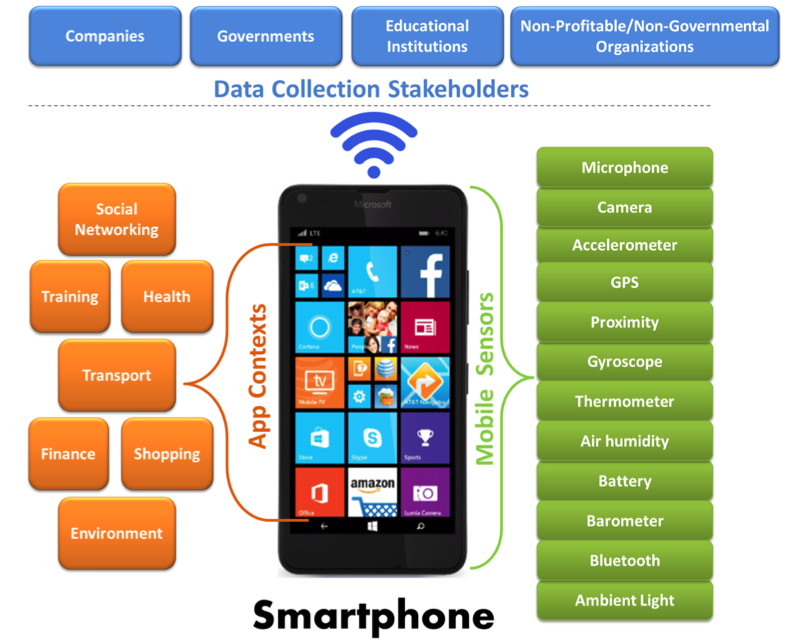
\includegraphics[width=\textwidth,keepaspectratio]{./images/all_features}
\caption{The Three Features Examined}
\label{fig:all_features}
\end{figure}

As it can be seen in the figure, there were a lot of sub-features to choose from each feature.
Increasing the number of sub-features for each feature in the experiment in turn increases the number of data requests posed to the user. Additionally,
we wanted to gain insight into the perception of users on the three features. Hence the survey
was prepared to understand all of the above. Additionally, it can help us redesign some of the aspects of the experiment based on the
ambiguities found and user feedback. The participants pool consist of both people who are aware and unaware of data privacy and sensors. Participants were not paid for filling out the survey. Till now, 199 entries have been recorded.

\subsection{Sub-Features}

\begin{figure}[ht!]
\centering
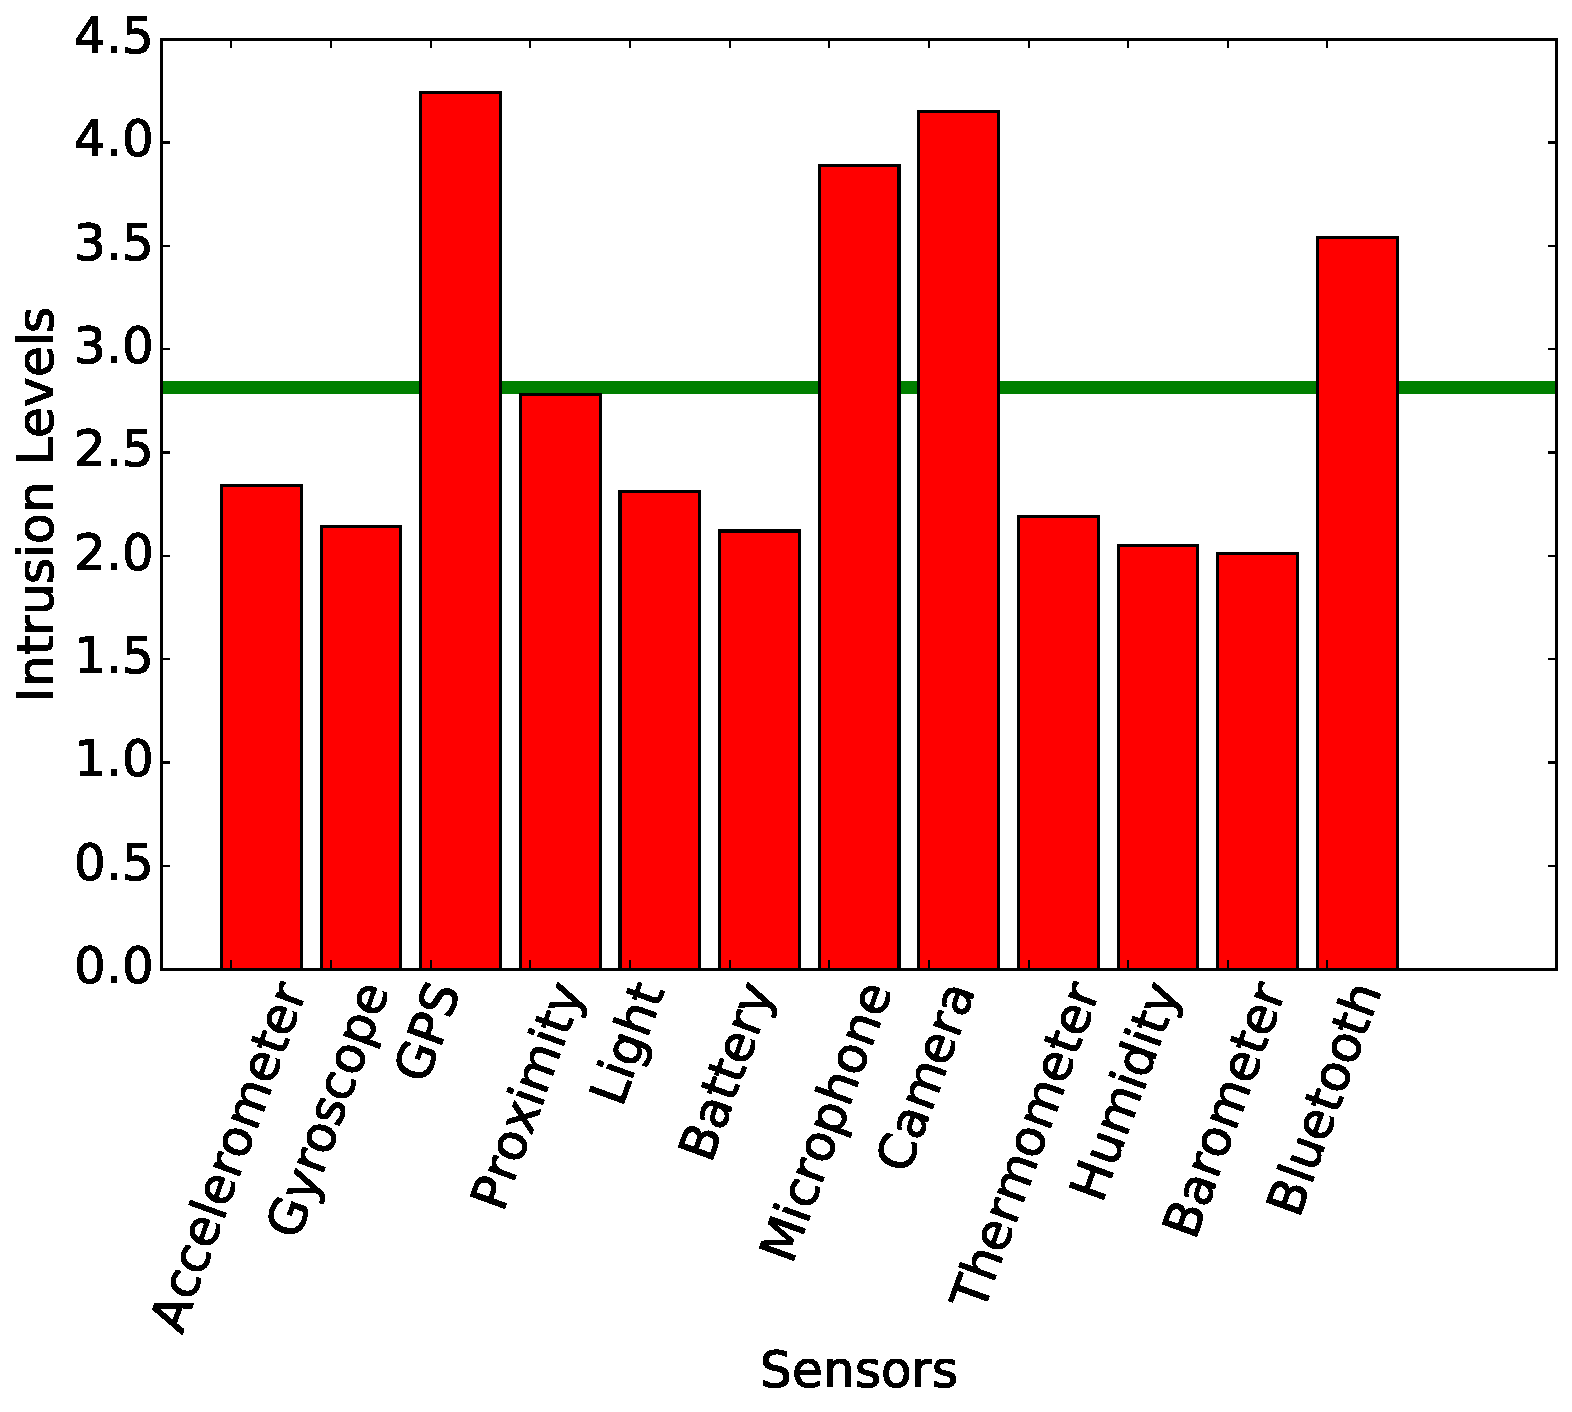
\includegraphics[width=\textwidth,keepaspectratio]{./images/pre_se}
\caption{Average Intrusion of Sensors Sub-Features}
\label{fig:pre_se}
\end{figure}

\begin{figure}[ht!]
\centering
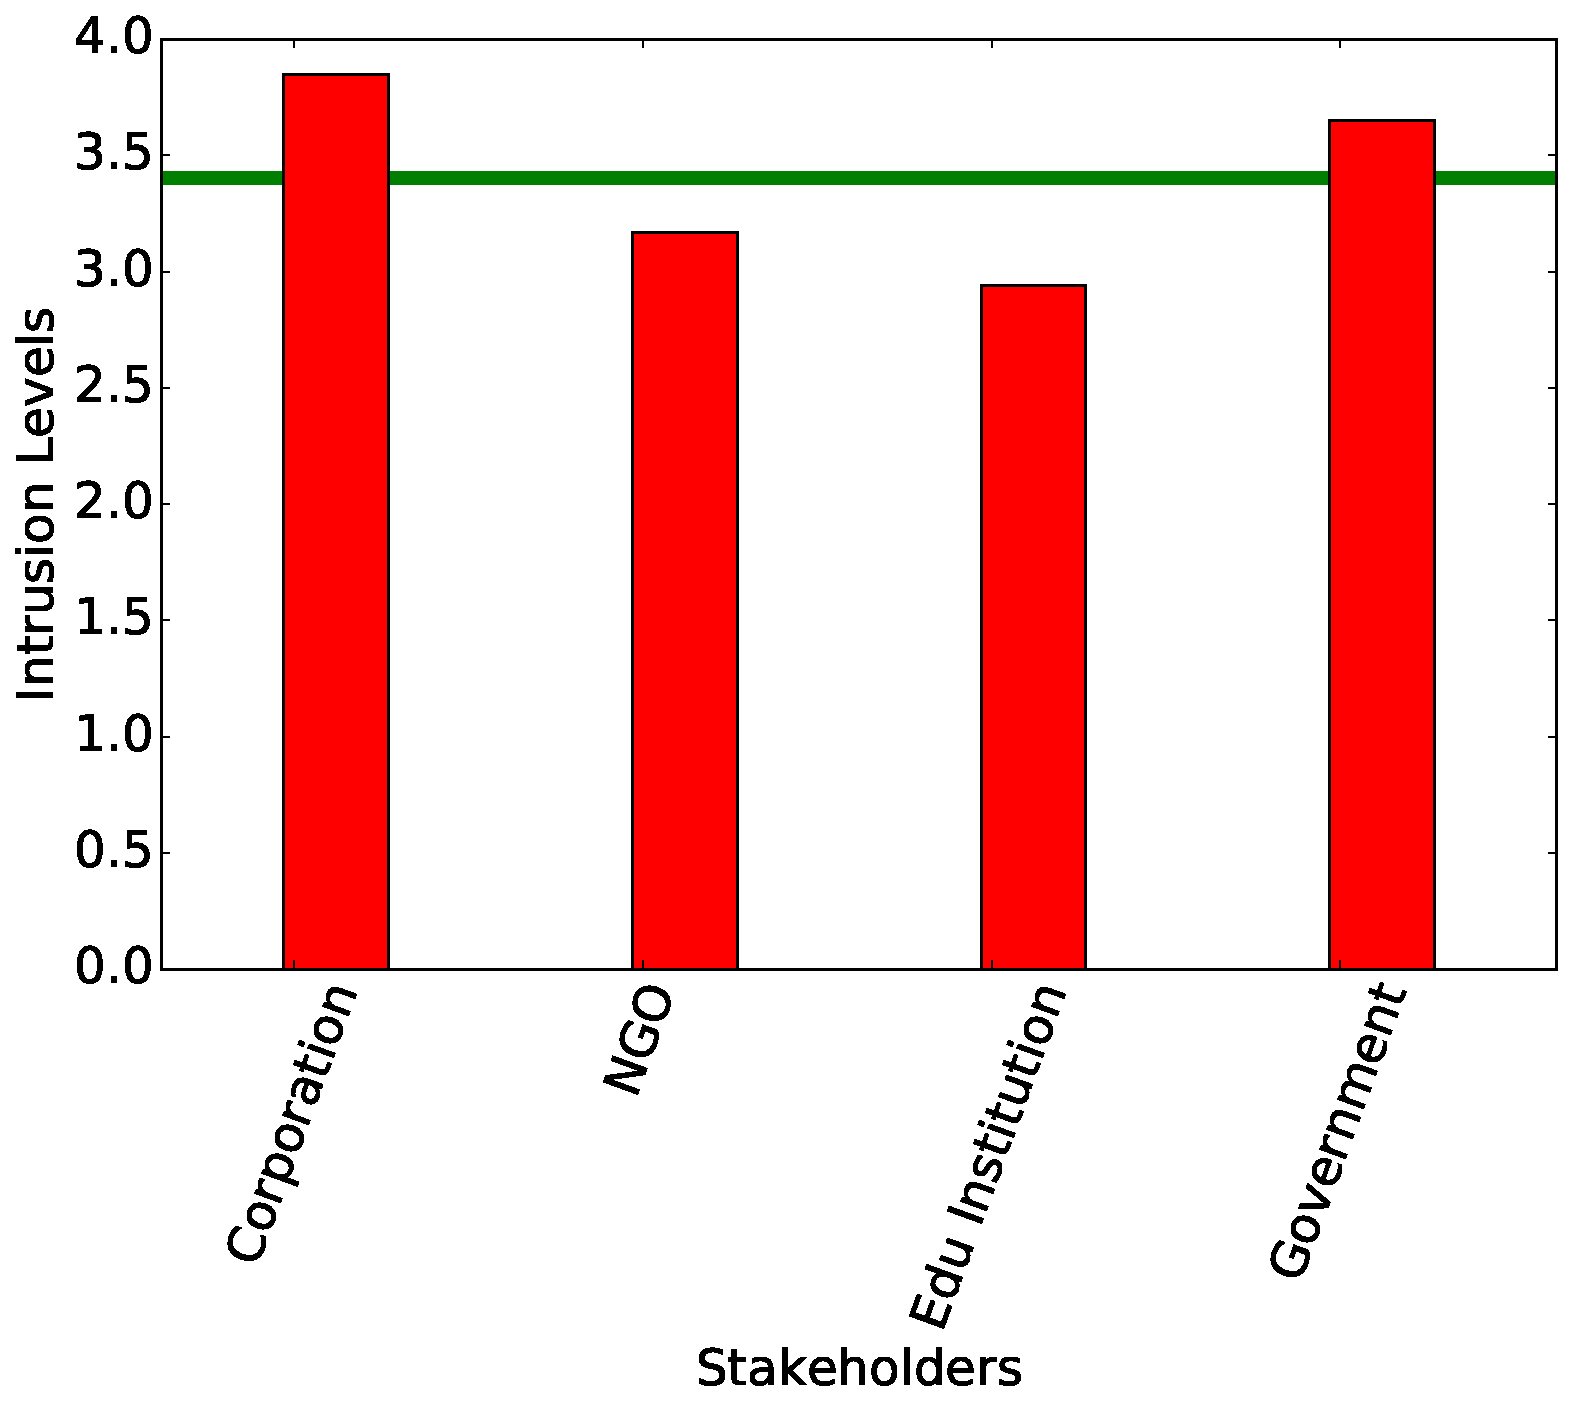
\includegraphics[width=\textwidth,height=0.7\textwidth,keepaspectratio]{./images/pre_st}
\caption{Average Intrusion of Stakeholders Sub-Features}
\label{fig:pre_st}
\end{figure}

\begin{figure}[ht!]
\centering
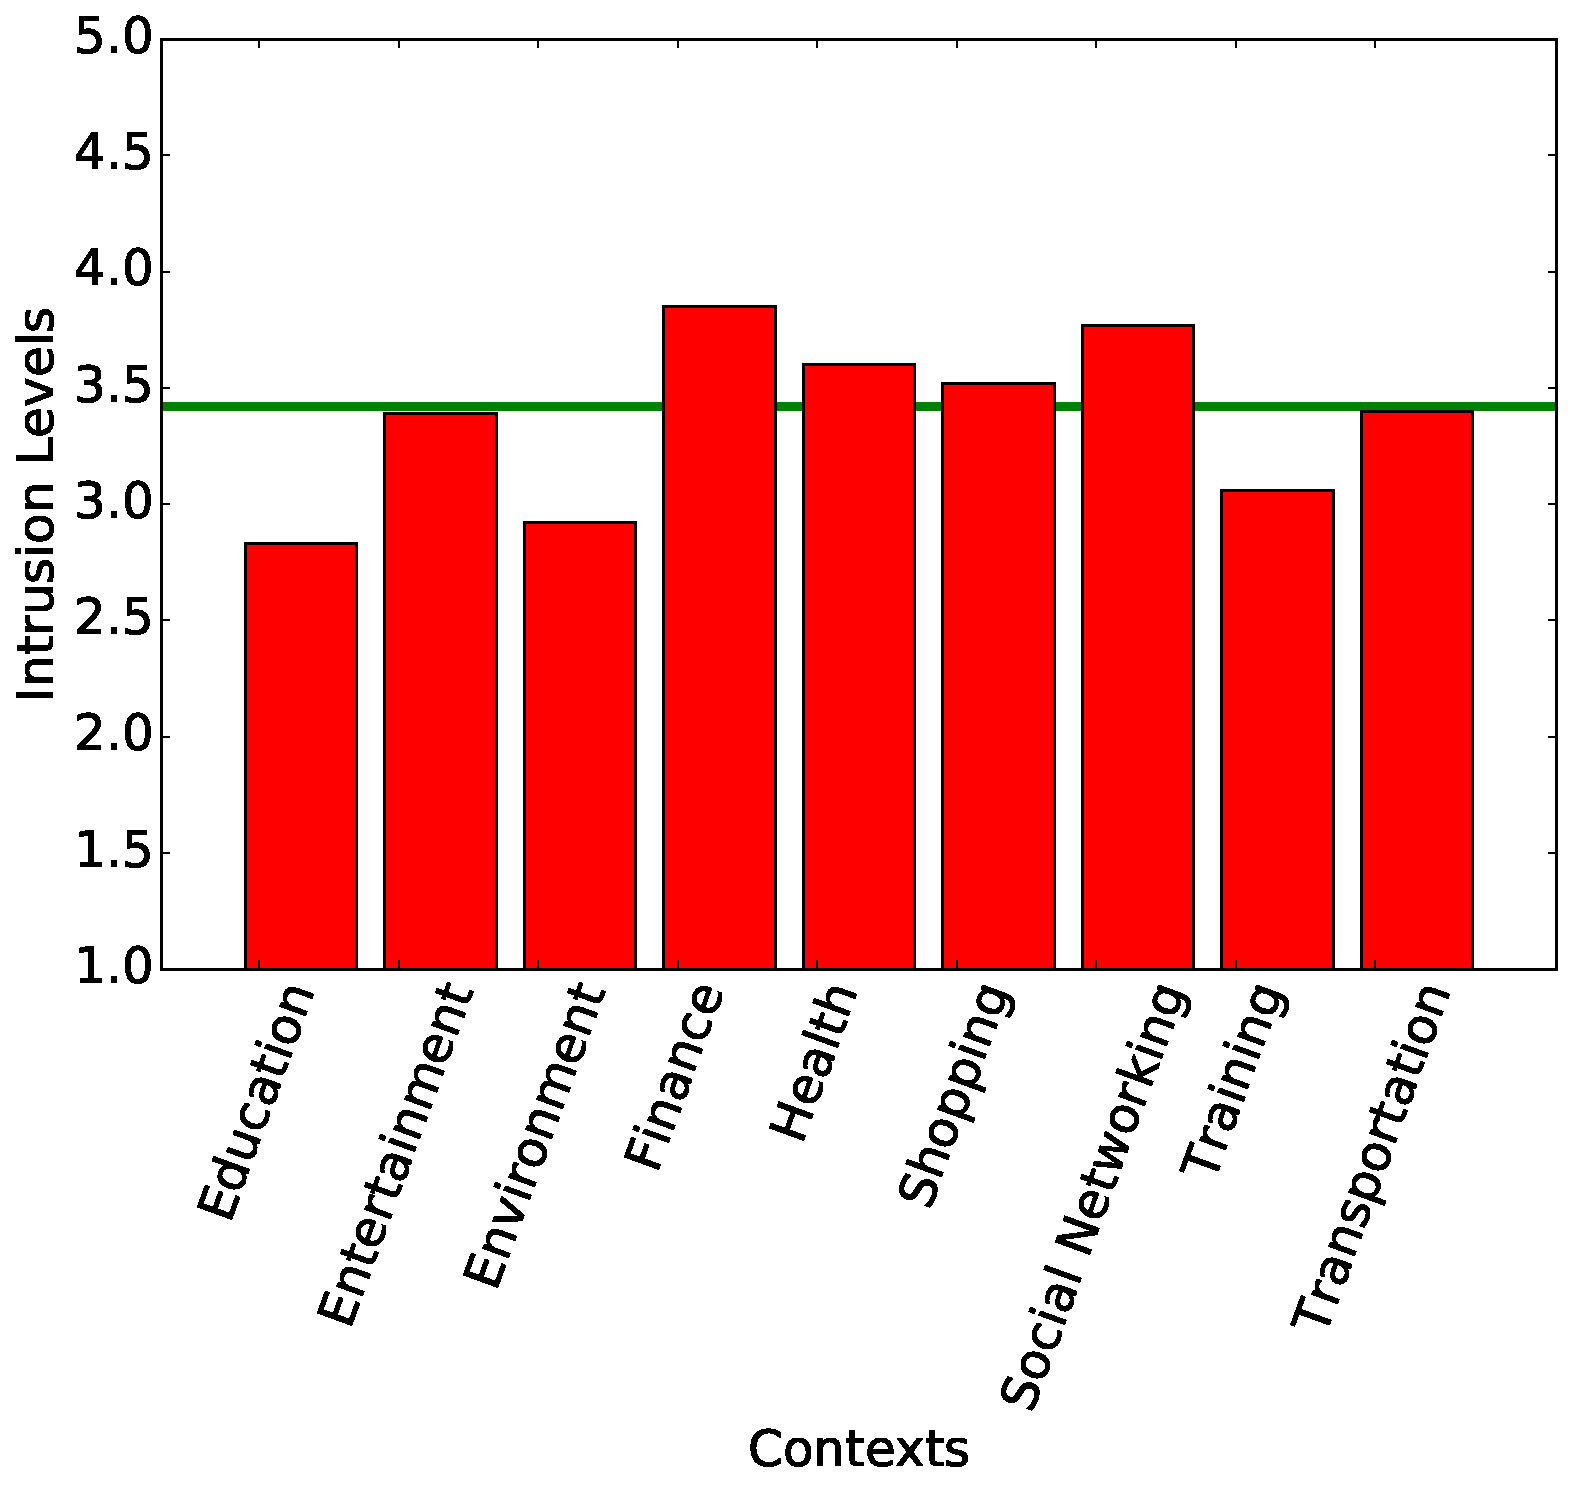
\includegraphics[width=\textwidth,keepaspectratio]{./images/pre_co}
\caption{Average Intrusion of Contexts Sub-Features}
\label{fig:pre_co}
\end{figure}

Figures \ref{fig:pre_se}, \ref{fig:pre_st} and \ref{fig:pre_co}, each show the average intrusion level of each possible sub-feature for
the sensors, stakeholders and contexts. For the experiment, it was decided to choose for each feature two non-intrusive and two intrusive sub-features
each. The minimum privacy intrusion level is one which indicates this sub-feature to not be intrusive, and the maximum is five which means that the sub-feature is very privacy intrusive.

For the sensors feature, it can be observed that the sub-features GPS and microphone are found to be have an intrusion of 4.2 and 3.8, which means users find these sensors on average very intrusive. On the other hand, sub-features light and accelerometer are found to be lower in intrusion with values of 2.2 and 2.3, which means that users find these sensors non-intrusive in general. The average of all sensors intrusion values is 2.8 as indicated by the blue line.

Similarly, looking at the stakeholder feature graph \ref{fig:pre_st}, it is seen that sub-features  corporation and government are found to be intrusive by the users with levels 3.8 and 3.6. On the other hand, sub-features educational institution and non governmental organization are found to be relatively less intrusive by the users with values of 3.2 and 2.95. For intrusion levels of contexts feature in graph \ref{fig:pre_co}, it is observed that sub-features social-networking and health are found to be intrusive by the users with values 3.8 and 3.6. Sub-features environment and
transportation are regarded as less intrusive by user with values of 2.9 and 3.3.The above mentioned sub-features for every feature have been chosen for the experiment.


\subsection{Privacy Options} \label{options}

Each data request is accompanied with privacy options ranging from $1$ to $5$ as explained in section \ref{o}. Option $1$ indicates that the users would like to
share their raw data without any sort of summarization or reduction in information. Option number $5$ indicates that the users would not like to share their data for this data request.
The options in between have linearly scaled summarization levels assigned to them ranging from least privacy ($1$) to most privacy ($5$). For more information on the summarization levels for each option please refer to section \ref{summa}. 

\subsection{Question Structure}

A data request is when a stakeholder asks users mobile sensor data for a particular context or purpose. Each data request to the user is posed in the form of a question with the following template :

\textit{"Please choose the amount of \underline{X} sensor type data shared with \underline{Y} stakeholder for use in a \underline{Z} context app"}

where Sensors X can be :
\begin{enumerate}
    \item Accelerometer
    \item Noise
    \item Location
    \item Light
\end{enumerate}
where Stakeholders Y can be:
\begin{enumerate}
    \item Corporation
    \item Educational Institution
    \item Non Governmental Organization
    \item Government
\end{enumerate}
and where Contexts Z can be:
\begin{enumerate}
    \item Environment
    \item Health/Fitness
    \item Navigation
    \item Social Networking
\end{enumerate}

In total this makes 64 data requests to the user. From now on, we will refer to mobile sensor data as just data.

\subsection{Budget and Experiment Duration}


The experiment is set to run for a total of two days, excluding the time taken for the entry phase and exit phase.
The budget set for the core phase of the experiment is $b=35$ Chf and is excluding the cost of participation
in the entry and exit phase. Participants are paid 10 Chf for coming to the Entry Phase, and 15 Chf for
participating in it. Similarly for the Exit Phase, participants are given 10 Chf for showing up, and 5 Chf for participating in it.
Out of the budget $B$, $\frac{1}{7}$ is given away for the participation of the users in the core phase.


\section{Entry Phase}
The entry phase denotes the first day of the experiment. Users are asked to install the application from the PlayStore. 

\subsection{Collecting General User Information}
As the figure \ref{fig:ui} shows, the users are asked to answer some personal non-intrusive questions. The following is asked from the users: 
\begin{enumerate}
    \item Gender
    \item Employment Status
    \item Education Level
    \item Year of birth
    \item Country where user has lived most of his life
    \item How many time a day do you check your Mobile phone per day.
    \item Kind of applications the user has in the mobile phone.
\end{enumerate}

\begin{figure}[htp]
  \subtop[User Information Screen 1\label{}]{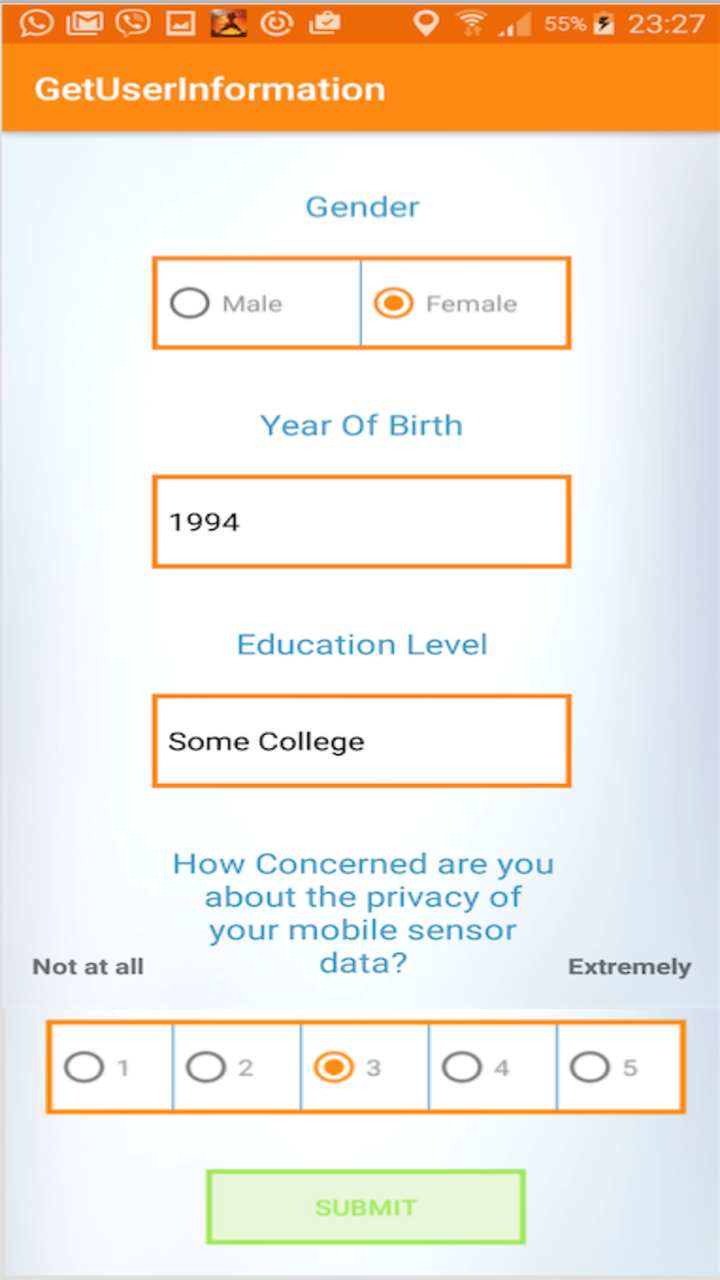
\includegraphics[width=0.45\linewidth,height=0.8\linewidth]{./images/ui_1_3}}\hspace{2em}
  \subtop[User Information Screen 2 \label{}]{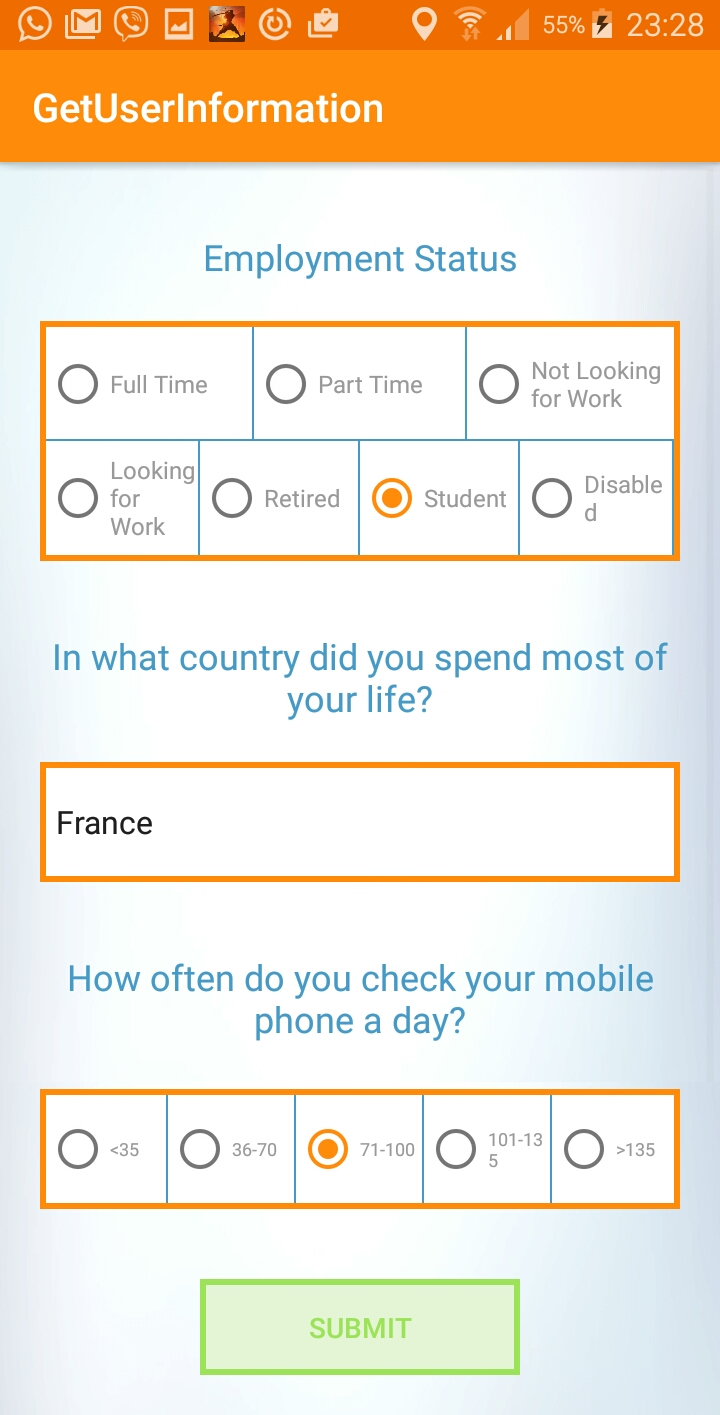
\includegraphics[width=0.45\linewidth,height=0.8\linewidth]{./images/ui_2_3}}%
  \caption{User Information Screens}
  \label{fig:ui}
\end{figure}

The users may go back and re-answer the questions, but once the submit button is pressed on the screen \ref{fig:ui3}, the data is sent to the server
and hence cannot be changed. Users cannot navigate to the next pages without filling out all the questions.

\subsection{Categorization of Features} \label{cat_feature}

As described in chapter \ref{model}, the users are asked to categorize the features sensors, stakeholders and contexts. As shown in figure 
\ref{fig:cat_f}, each of the features are indicated followed by a drop down list of privacy options ranging from \textit{"very low privacy intrusion"} to \textit{"very privacy high privacy intrusion"}. The option \textit{"very low privacy intrusion"} means that the feature does not affect the users mobile sensor data sharing decision, whereas 
\textit{"very privacy high privacy intrusion"} refers to a feature that very much affects the sharing of mobile sensor data. 

Users need to click on the
drop down menu to choose one of the privacy intrusion options. All the options are compulsory, and no default option is provided. Users cannot navigate to the next page without filling out all of the questions.

\begin{figure}[htp]
  \subtop[Categorizing Features\label{fig:cat_f}]{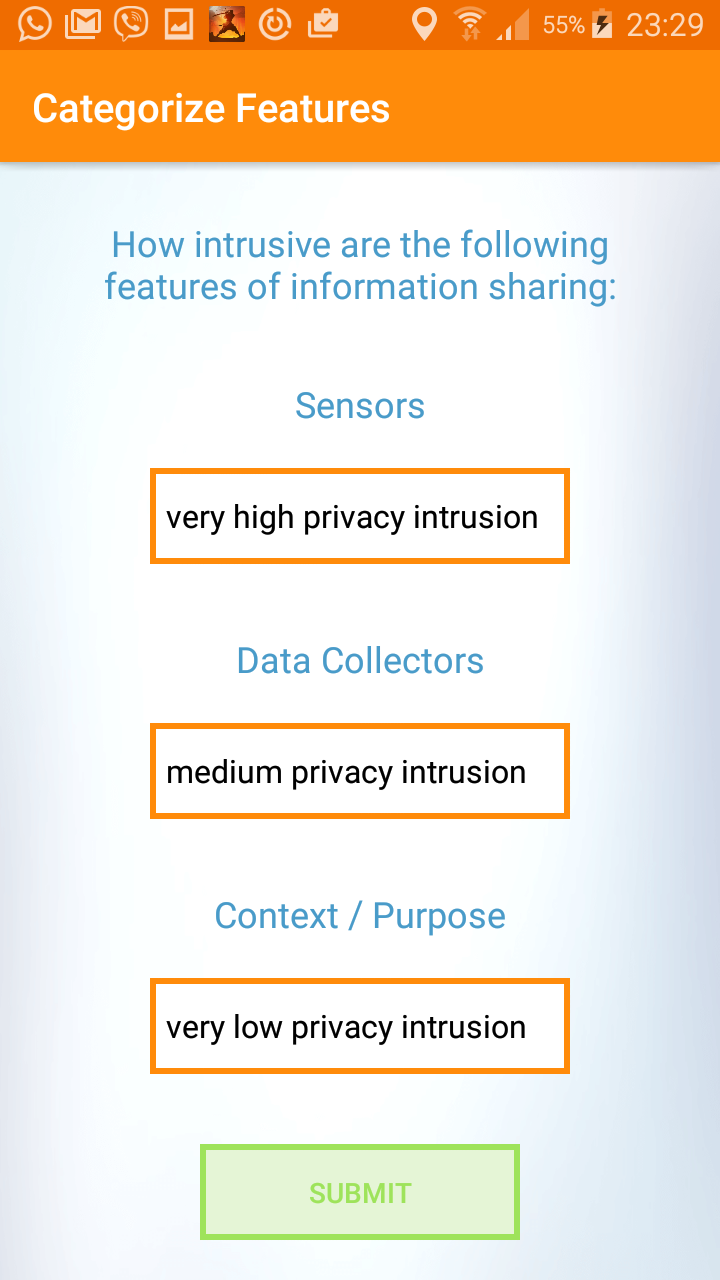
\includegraphics[width=0.4\linewidth, height=10cm]{./images/cat_features}}\hspace{1em}
  \subtop[User Information Screen 3 \label{fig:ui1}]{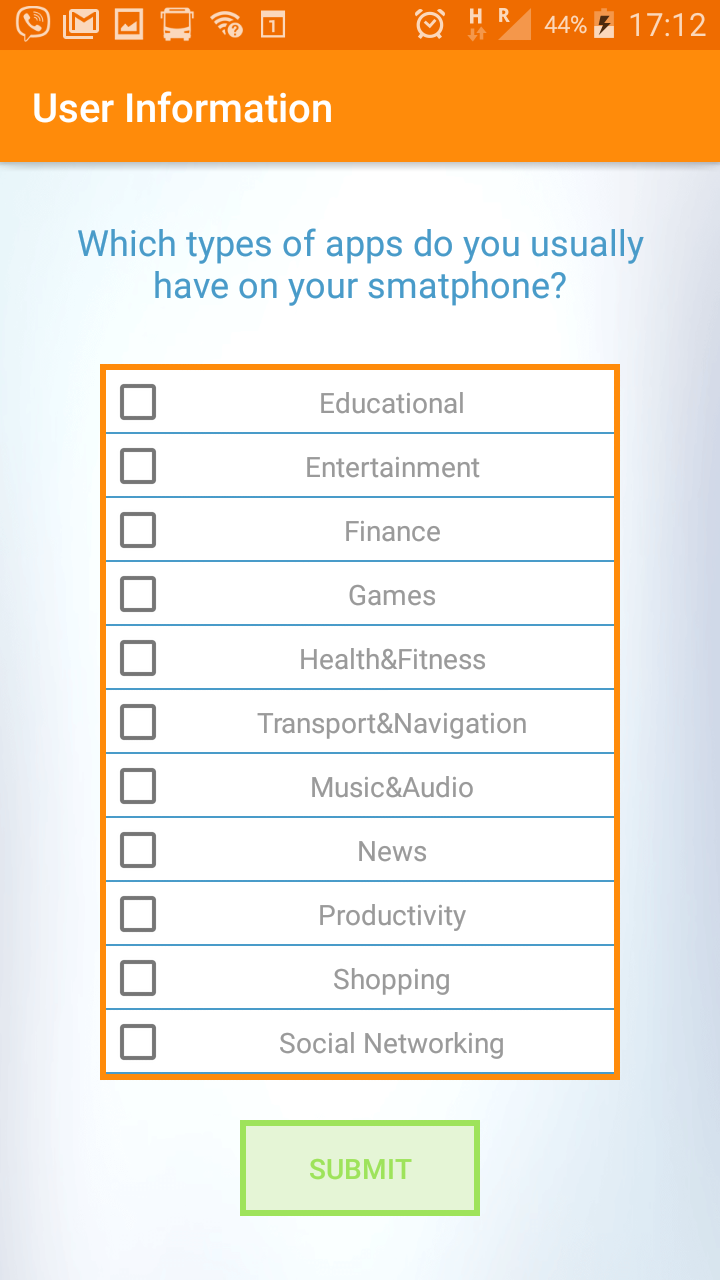
\includegraphics[width=0.4\linewidth, height=10cm]{./images/ui_checkboxes}}%
  \caption{Categorization and User Information Screens}
  \label{fig:cat}
\end{figure}

\subsection{Categorization of Sub-Features}
For each of the features categorized in the previous sub-section, their sub-features need to be categorized in a similar fashion. Once again,
the privacy options range from \textit{"very low privacy intrusion"} to \textit{"very high privacy intrusion"} like in section \ref{cat_feature} . The users are first presented with
the categorization of Sensors sub-features as shown in figure \ref{fig:cat_se}. 


Below each sensor is a drop down menu where the user can choose how much each of the sensors
would affect the mobile sensor data sharing. Once all the sensors have been associated with a privacy intrusion level, the user can click the green submit button and is directed to
the next page where the sub-features of stakeholders need to be in turn categorized in a similar fashion. This is depicted in
figure \ref{fig:cat_st}.

\begin{figure}[htp]
  \subtop[Categorizing Sensors\label{fig:cat_se}]{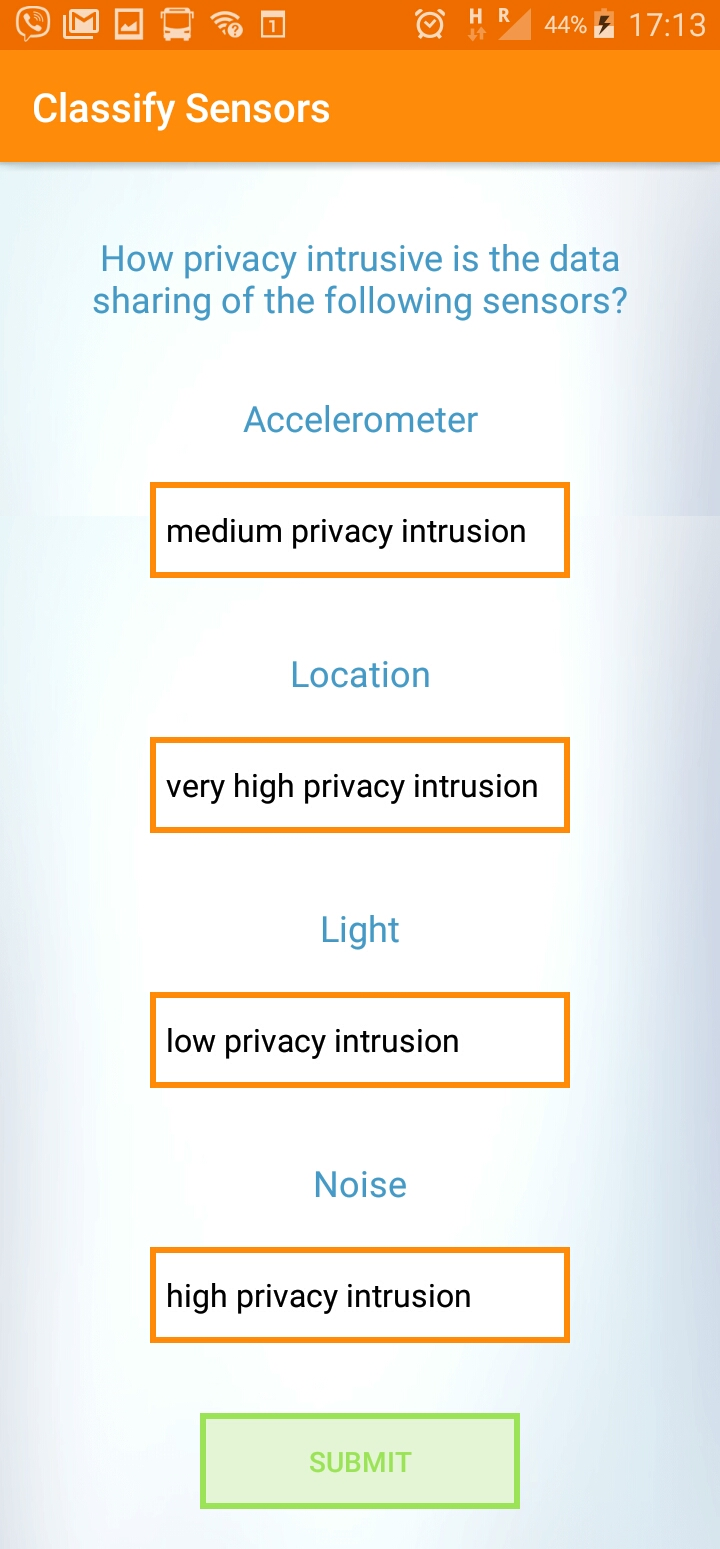
\includegraphics[width=0.4\linewidth, height=10cm]{./images/cat_sensors}}\hspace{1em}
  \subtop[Categorizing Stakeholders \label{fig:cat_st}]{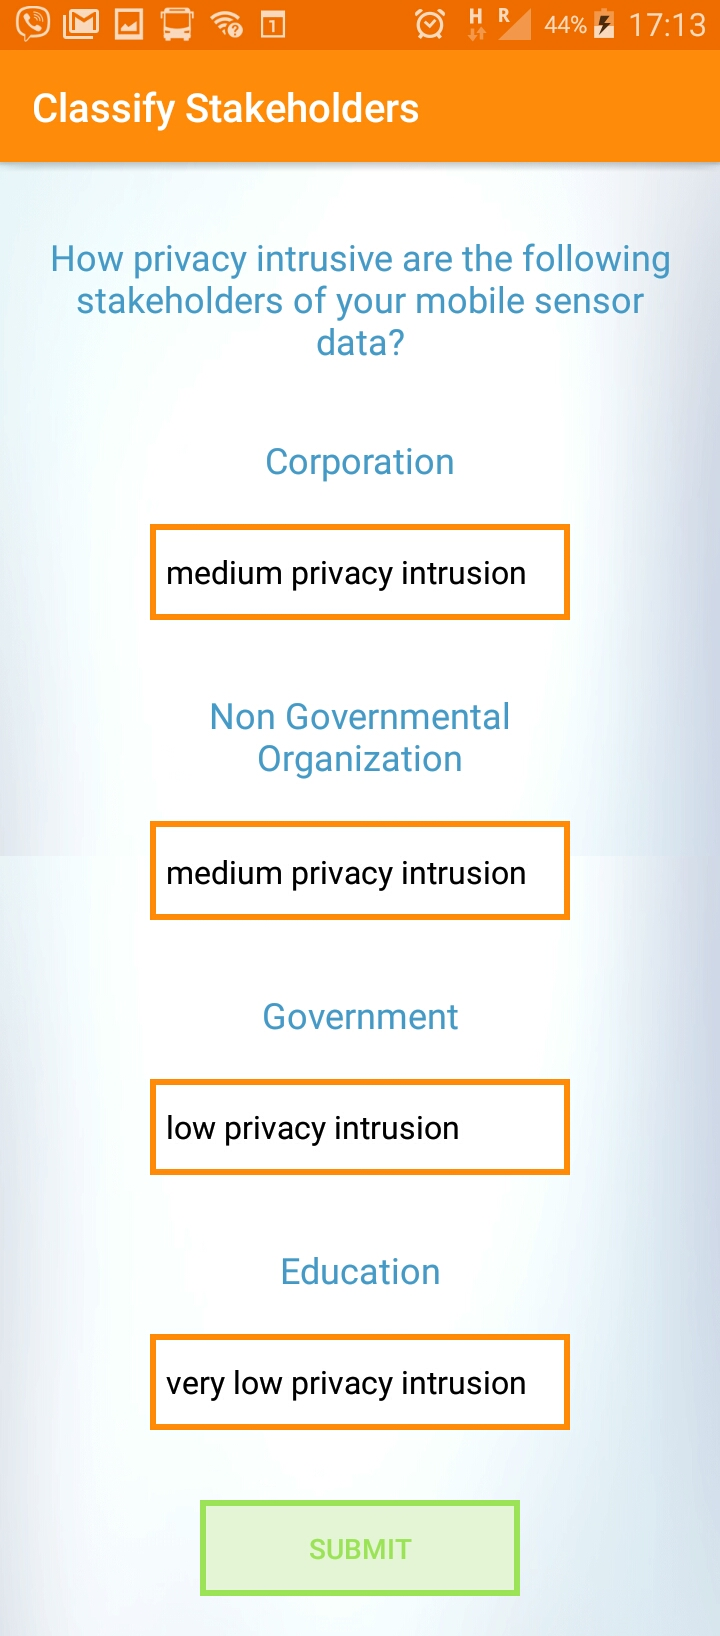
\includegraphics[width=0.4\linewidth, height=10cm]{./images/cat_stakeholders}}%
  \caption{Categorization of Sensors and Stakeholders Screen}
  \label{fig:cat1}
\end{figure}

\begin{figure}[ht!]
\centering
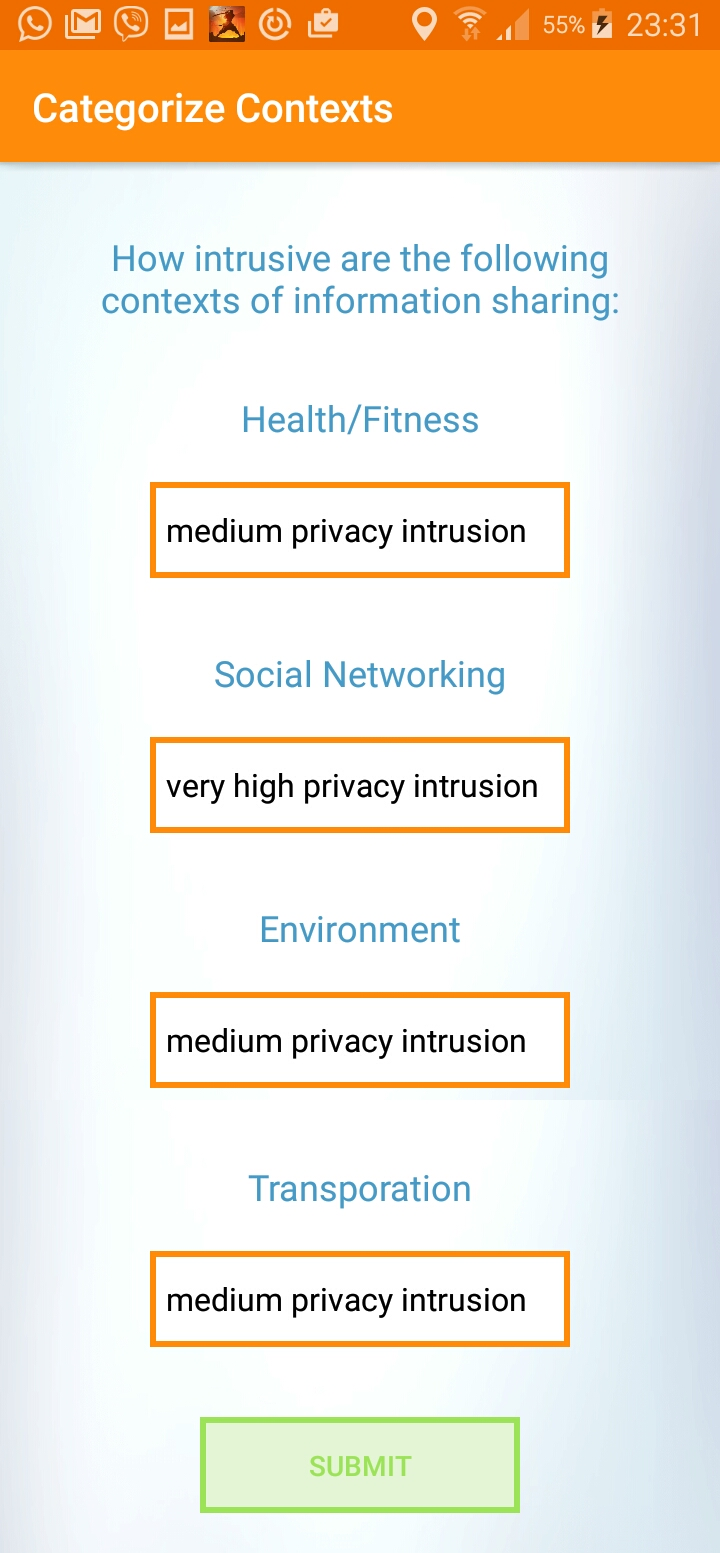
\includegraphics[width=0.4\linewidth, height=10cm]{./images/cat_contexts}
\caption{Categorization of Contexts Screen}
\label{fig:cat_co}
\end{figure}

Each stakeholder type has a drop
down menu each where the user can once again classify how much each of them affect data sharing.
Once the user has finished entering the privacy intrusion level for stakeholders sub-features, the user can click the green submit button and is directed to the next page.


On this page, the users are asked to categorize how much each of the contexts sub-features affect mobile sensor data sharing. This is depicted in figure \ref{fig:cat_co}. Each context has a drop down menu below, where the user can rate each context. Once this has been done the user can click on the green submit button. The user will be redirected to the next page only if all the drop down boxes have been filled out. All questions are compulsory there is no default choice.

\subsection{Answering Questions with No Incentives}  \label{quest_wi}
After the categorization questions are answered and user answers are recorded, users will be presented with 64 questions. Each of these questions is a mobile sensor data request
to the users. Users can choose from the available five privacy options mentioned in section \ref{options}. The options are indicated as a measure of how much data users can give, ranging from maximum data to least data. The higher the privacy of the option, the less information about the sensor data is given away for that request and vice versa. Users can change the answers for a data request until the green submit button on top of the options that appears is clicked. The screen with the data request is shown in figure \ref{fig:first_1}. 

After the users choose an option for the data request, a green submit button appears which is shown in figure \ref{fig:first_2}. Clicking on the submit button sends the response to the data request to the server and cannot be changed. At this stage, no indications of credit gained or privacy improvements are indicated.

\begin{figure}[htp]
  \subtop[Question Screen\label{fig:first_1}]{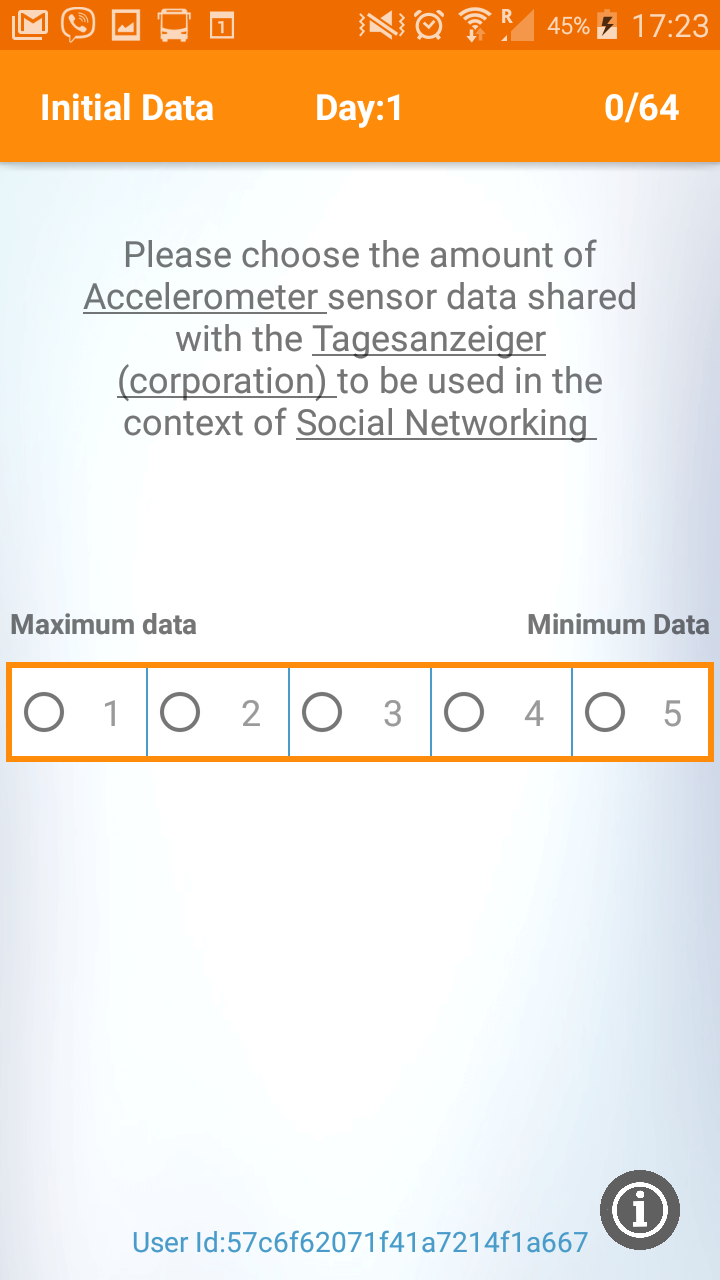
\includegraphics[width=0.5\linewidth]{./images/first_day_1}}\hspace{3em}
  \subtop[Question Screen with Submit button \label{fig:first_2}]{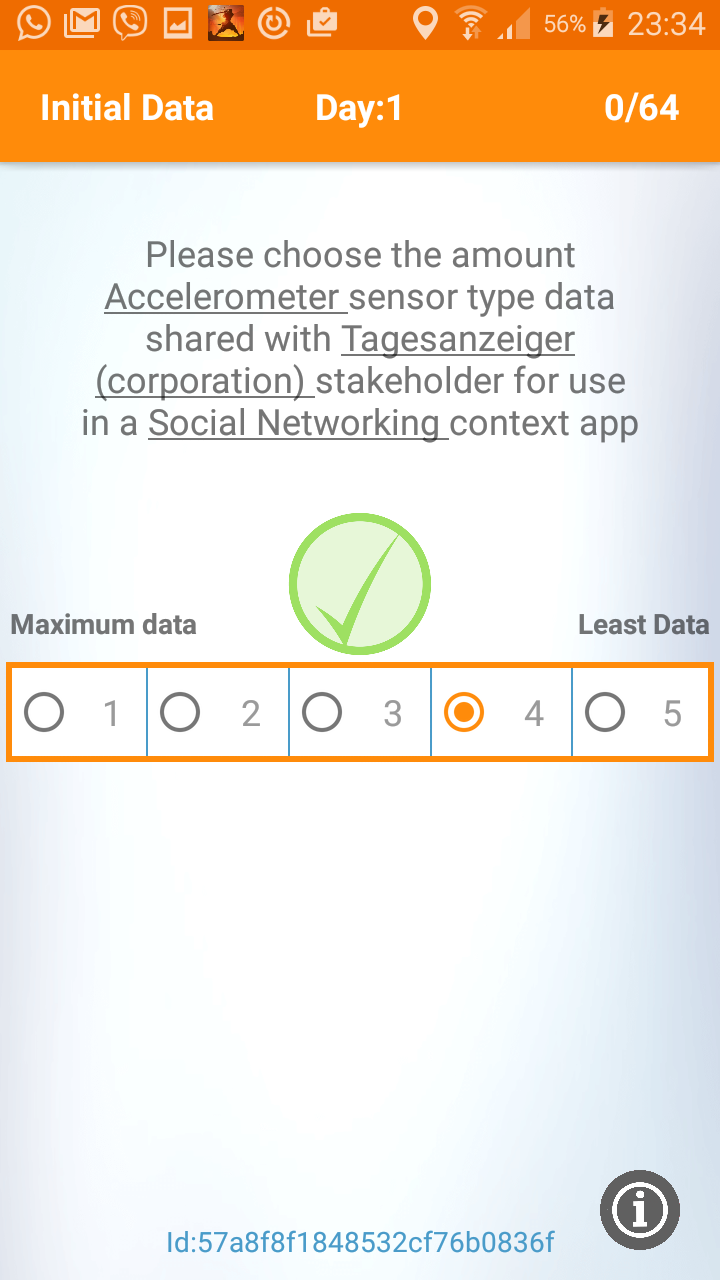
\includegraphics[width=0.5\linewidth]{./images/first_day_2}}%
  \caption{First Day Screen}
  \label{fig:first}
\end{figure}


Once all the questions have been answered, the user goes to the core phase of the experiment, which starts at day number two. In the experiment, day number one is the entry phase, the core phase is day number two and three.

\section{Core Phase} \label{core}

%\begin{figure}[ht!]
%\centering
%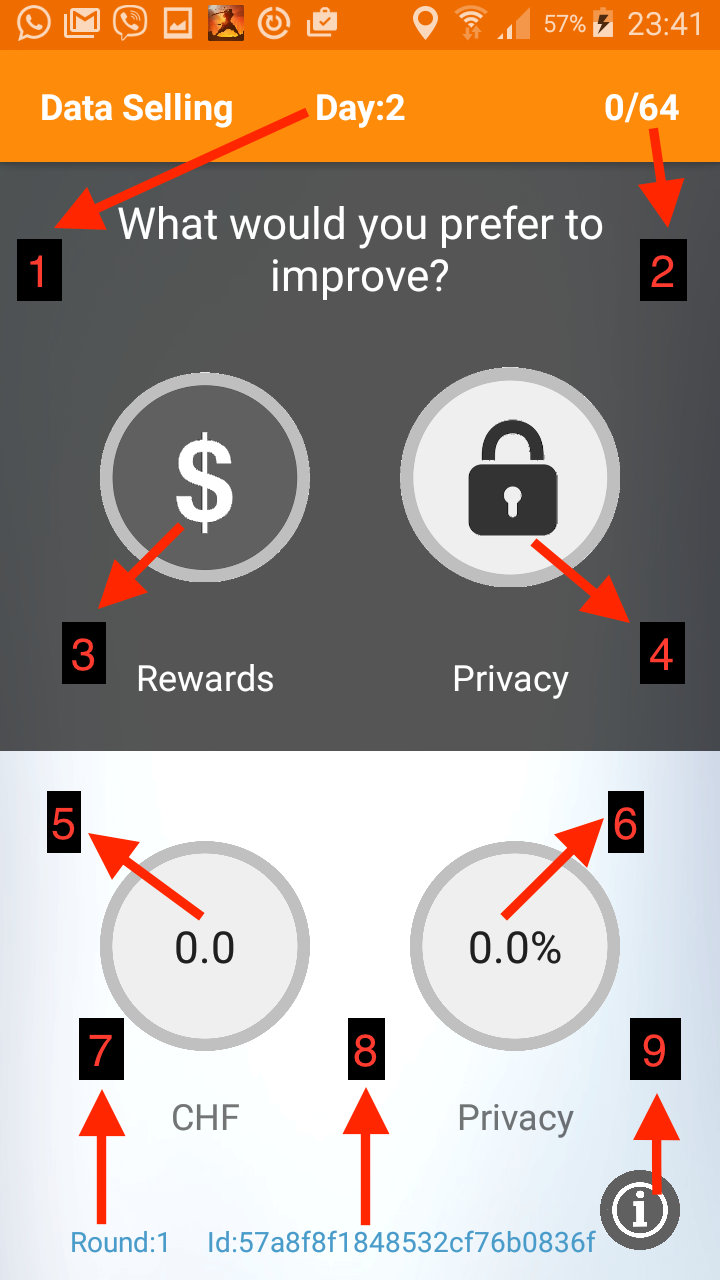
\includegraphics[width=\textwidth,keepaspectratio]{./images/improve}
%\caption{Improvement screen }
%\label{fig:imp}
%\end{figure}

\begin{figure}[htp]
  \subtop[\label{fig:imp_a}]{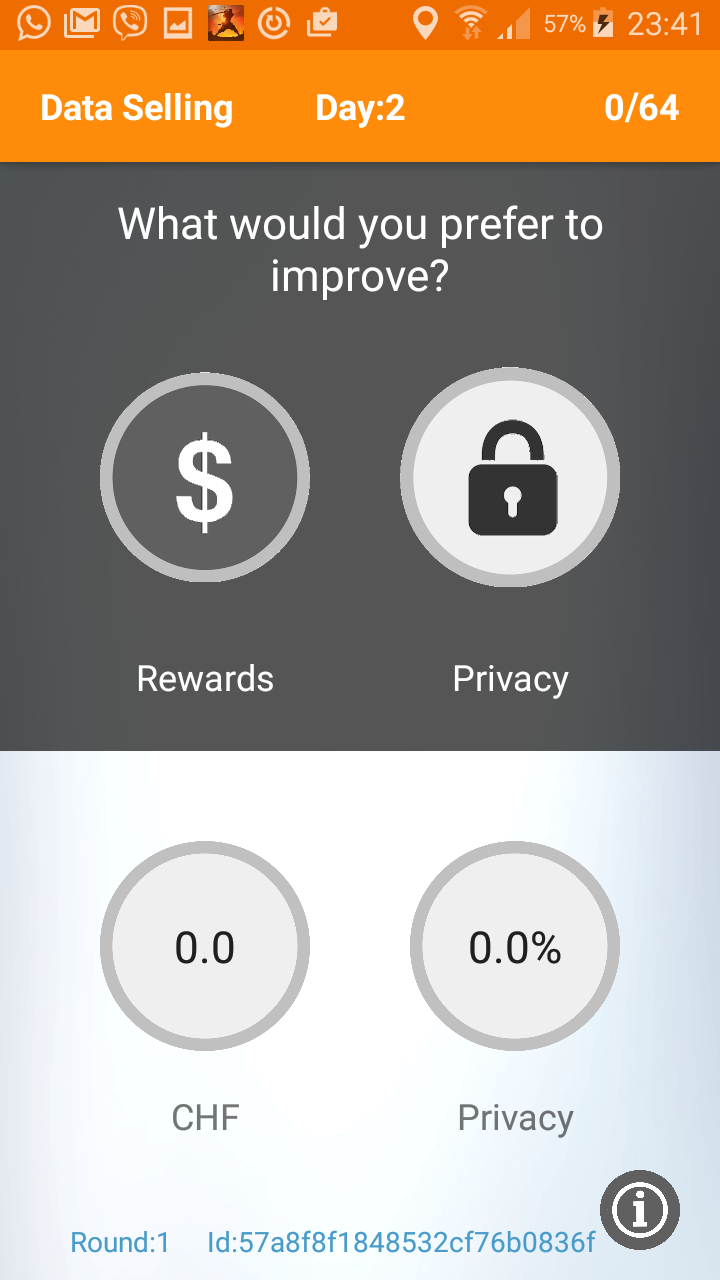
\includegraphics[width=0.45\linewidth]{./images/improve_layout}}\hspace{1em}
  \subtop[\label{fig:imp_wa}]{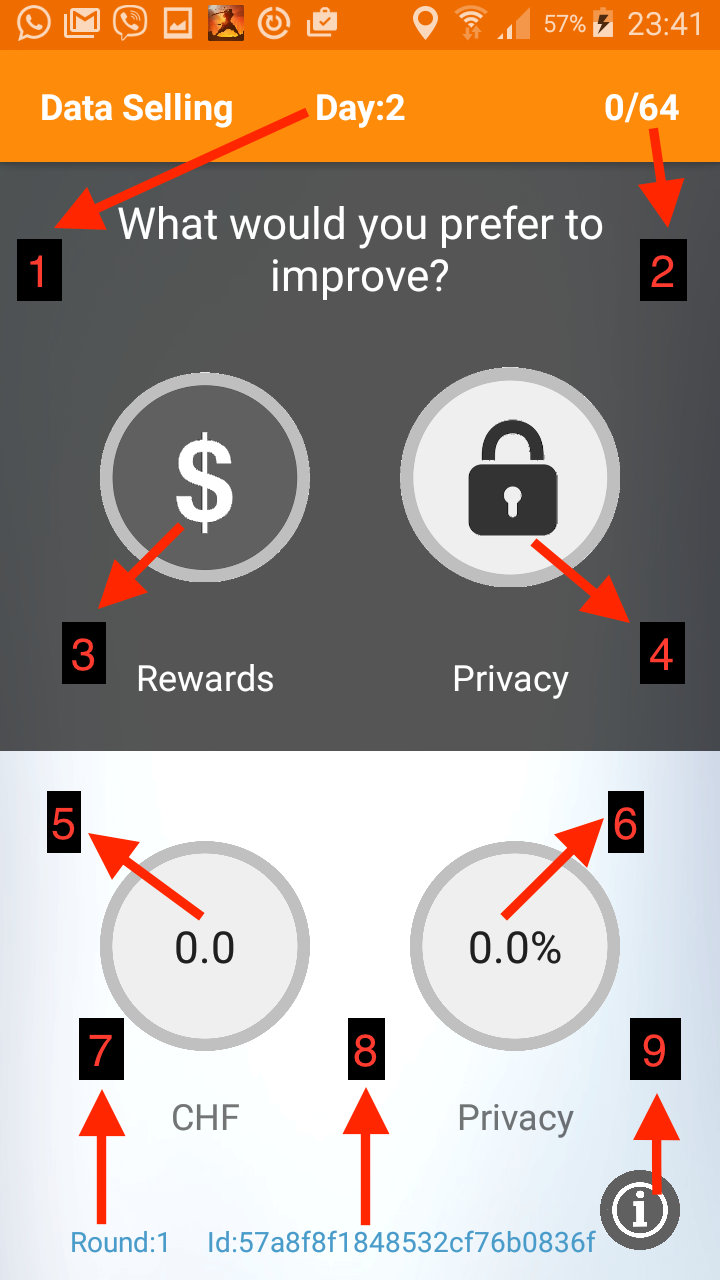
\includegraphics[width=0.45\linewidth]{./images/improve}}%
  \caption{Improvement screen}
  \label{fig:imp}
\end{figure}

Once the entry phase is done, the user is presented with the screen shown in figure \ref{imp}.
The {\it "i"} button at the bottom right of the screen denoted by the number 9 is clickable. This takes the users to the FairDataShare portal. Figure \ref{fig:fds_user_register} shows the homepage of the portal. Users can then click on the data generator registration section of the website where they can signup with their:

\begin{enumerate}
    \item Username
    \item Password
    \item Email
    \item Unique Identifier
\end{enumerate}

The unique identifier is located at the bottom of the application screen is an alphanumeric sequence denoted by number 8. If it is long pressed the user can select the identifier, then copy and paste it in the  textbox asking for the unique identifier in the portal. Figure \ref{fig:fds_user_register} shows what the registration page looks like.
The users can use this website to see all the data collected from them for all the mobile sensors. More details about the FairDataShare portal
refer to the section \ref{fds}.
%
%\begin{figure}[htp]
%  \subtop[FairDataShare Homepage\label{fig:fds_home}]{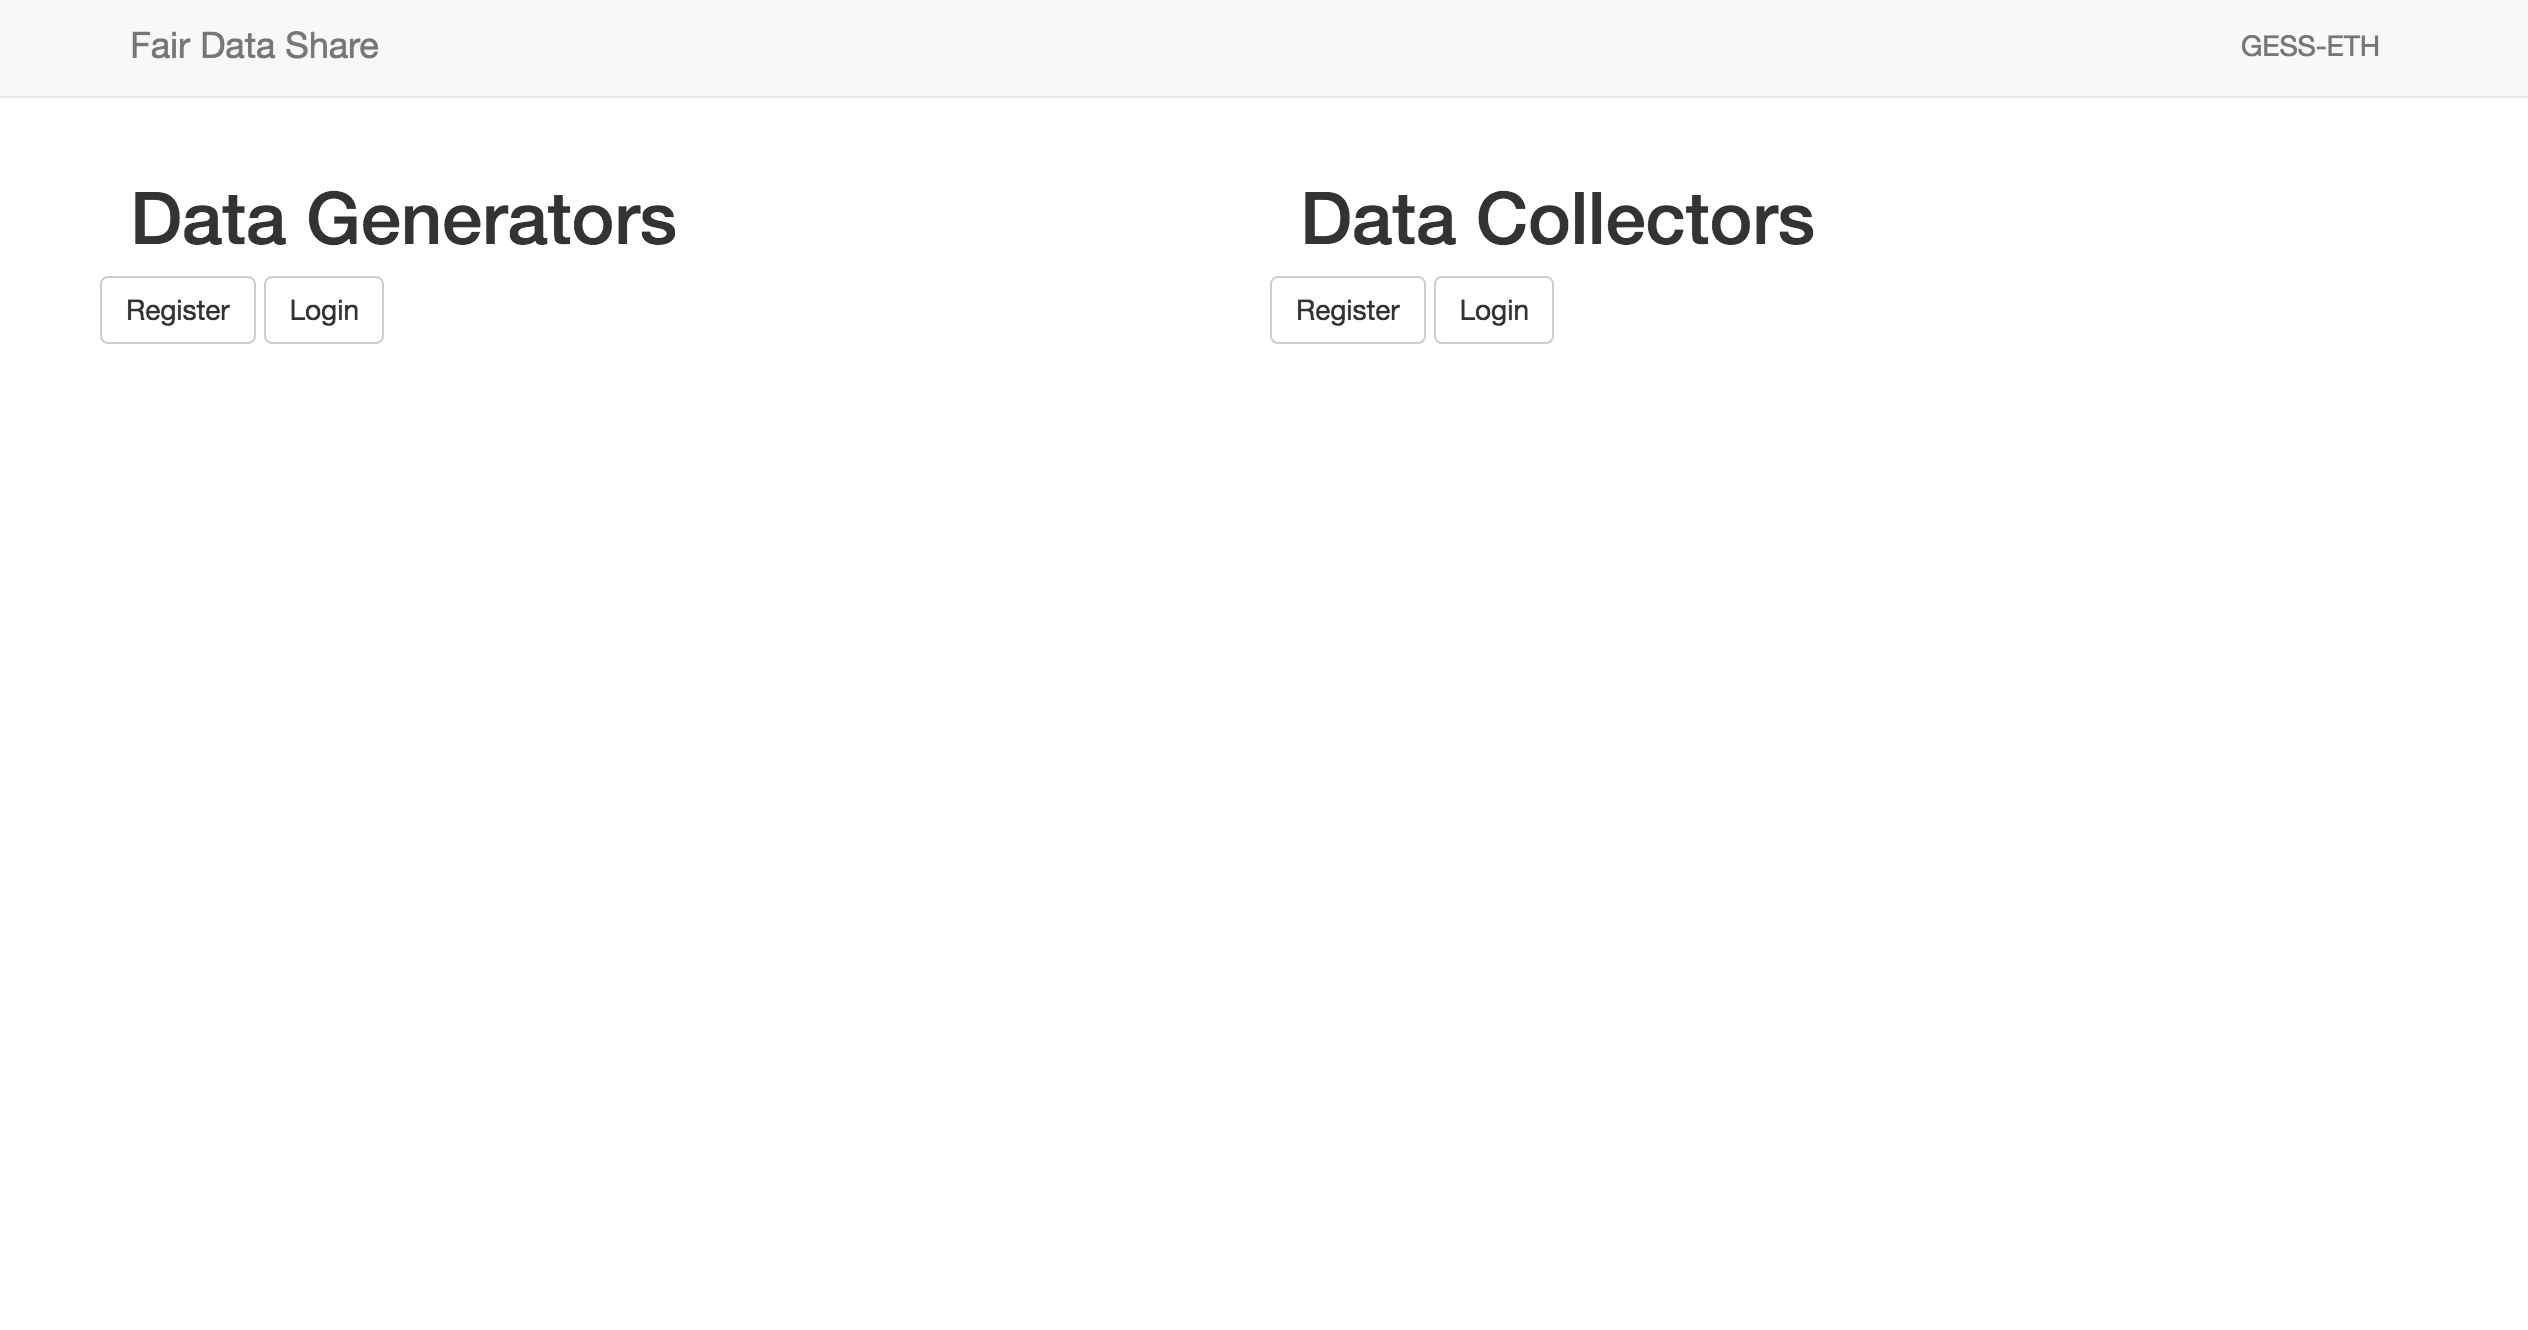
\includegraphics[width=0.4\linewidth]{./images/fds}}\hspace{1em}
%  \subtop[Data Generators Registration Page \label{fig:fds_user_register}]{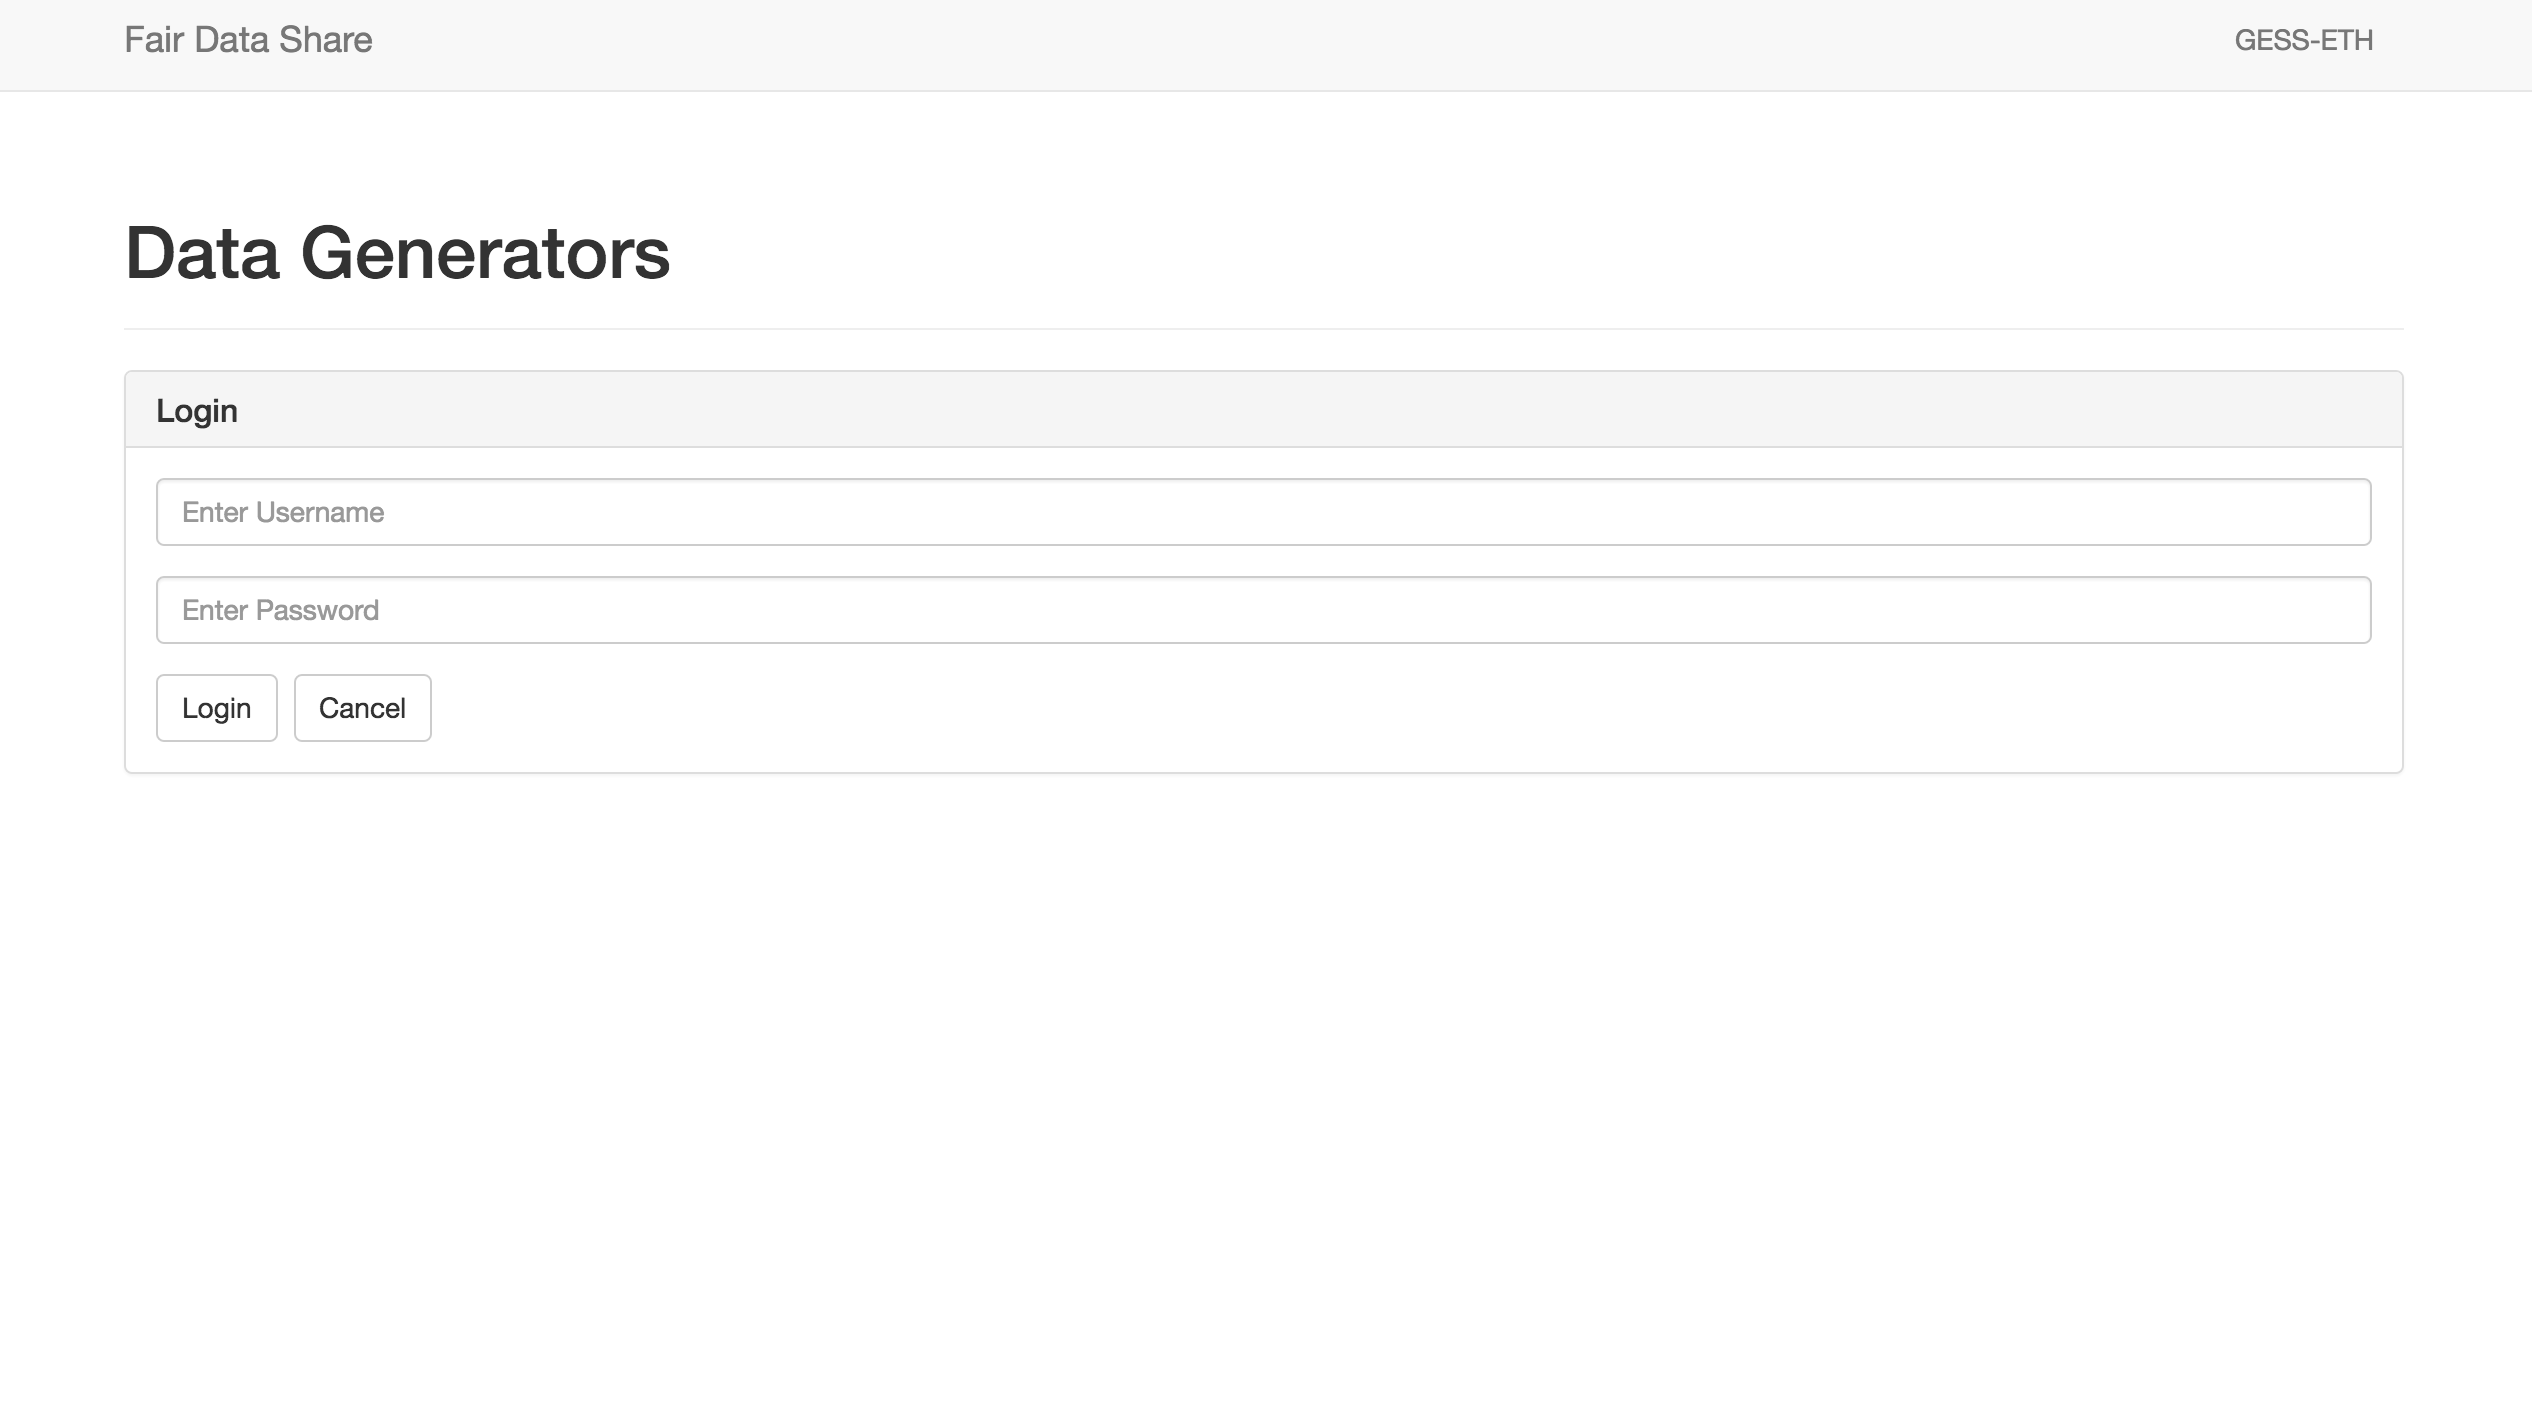
\includegraphics[width=0.4\linewidth]{./images/fds_user_login}}%
%  \caption{FairDataShare Portal}
%  \label{fig:first}
%\end{figure}

\begin{figure}[ht!]
\centering
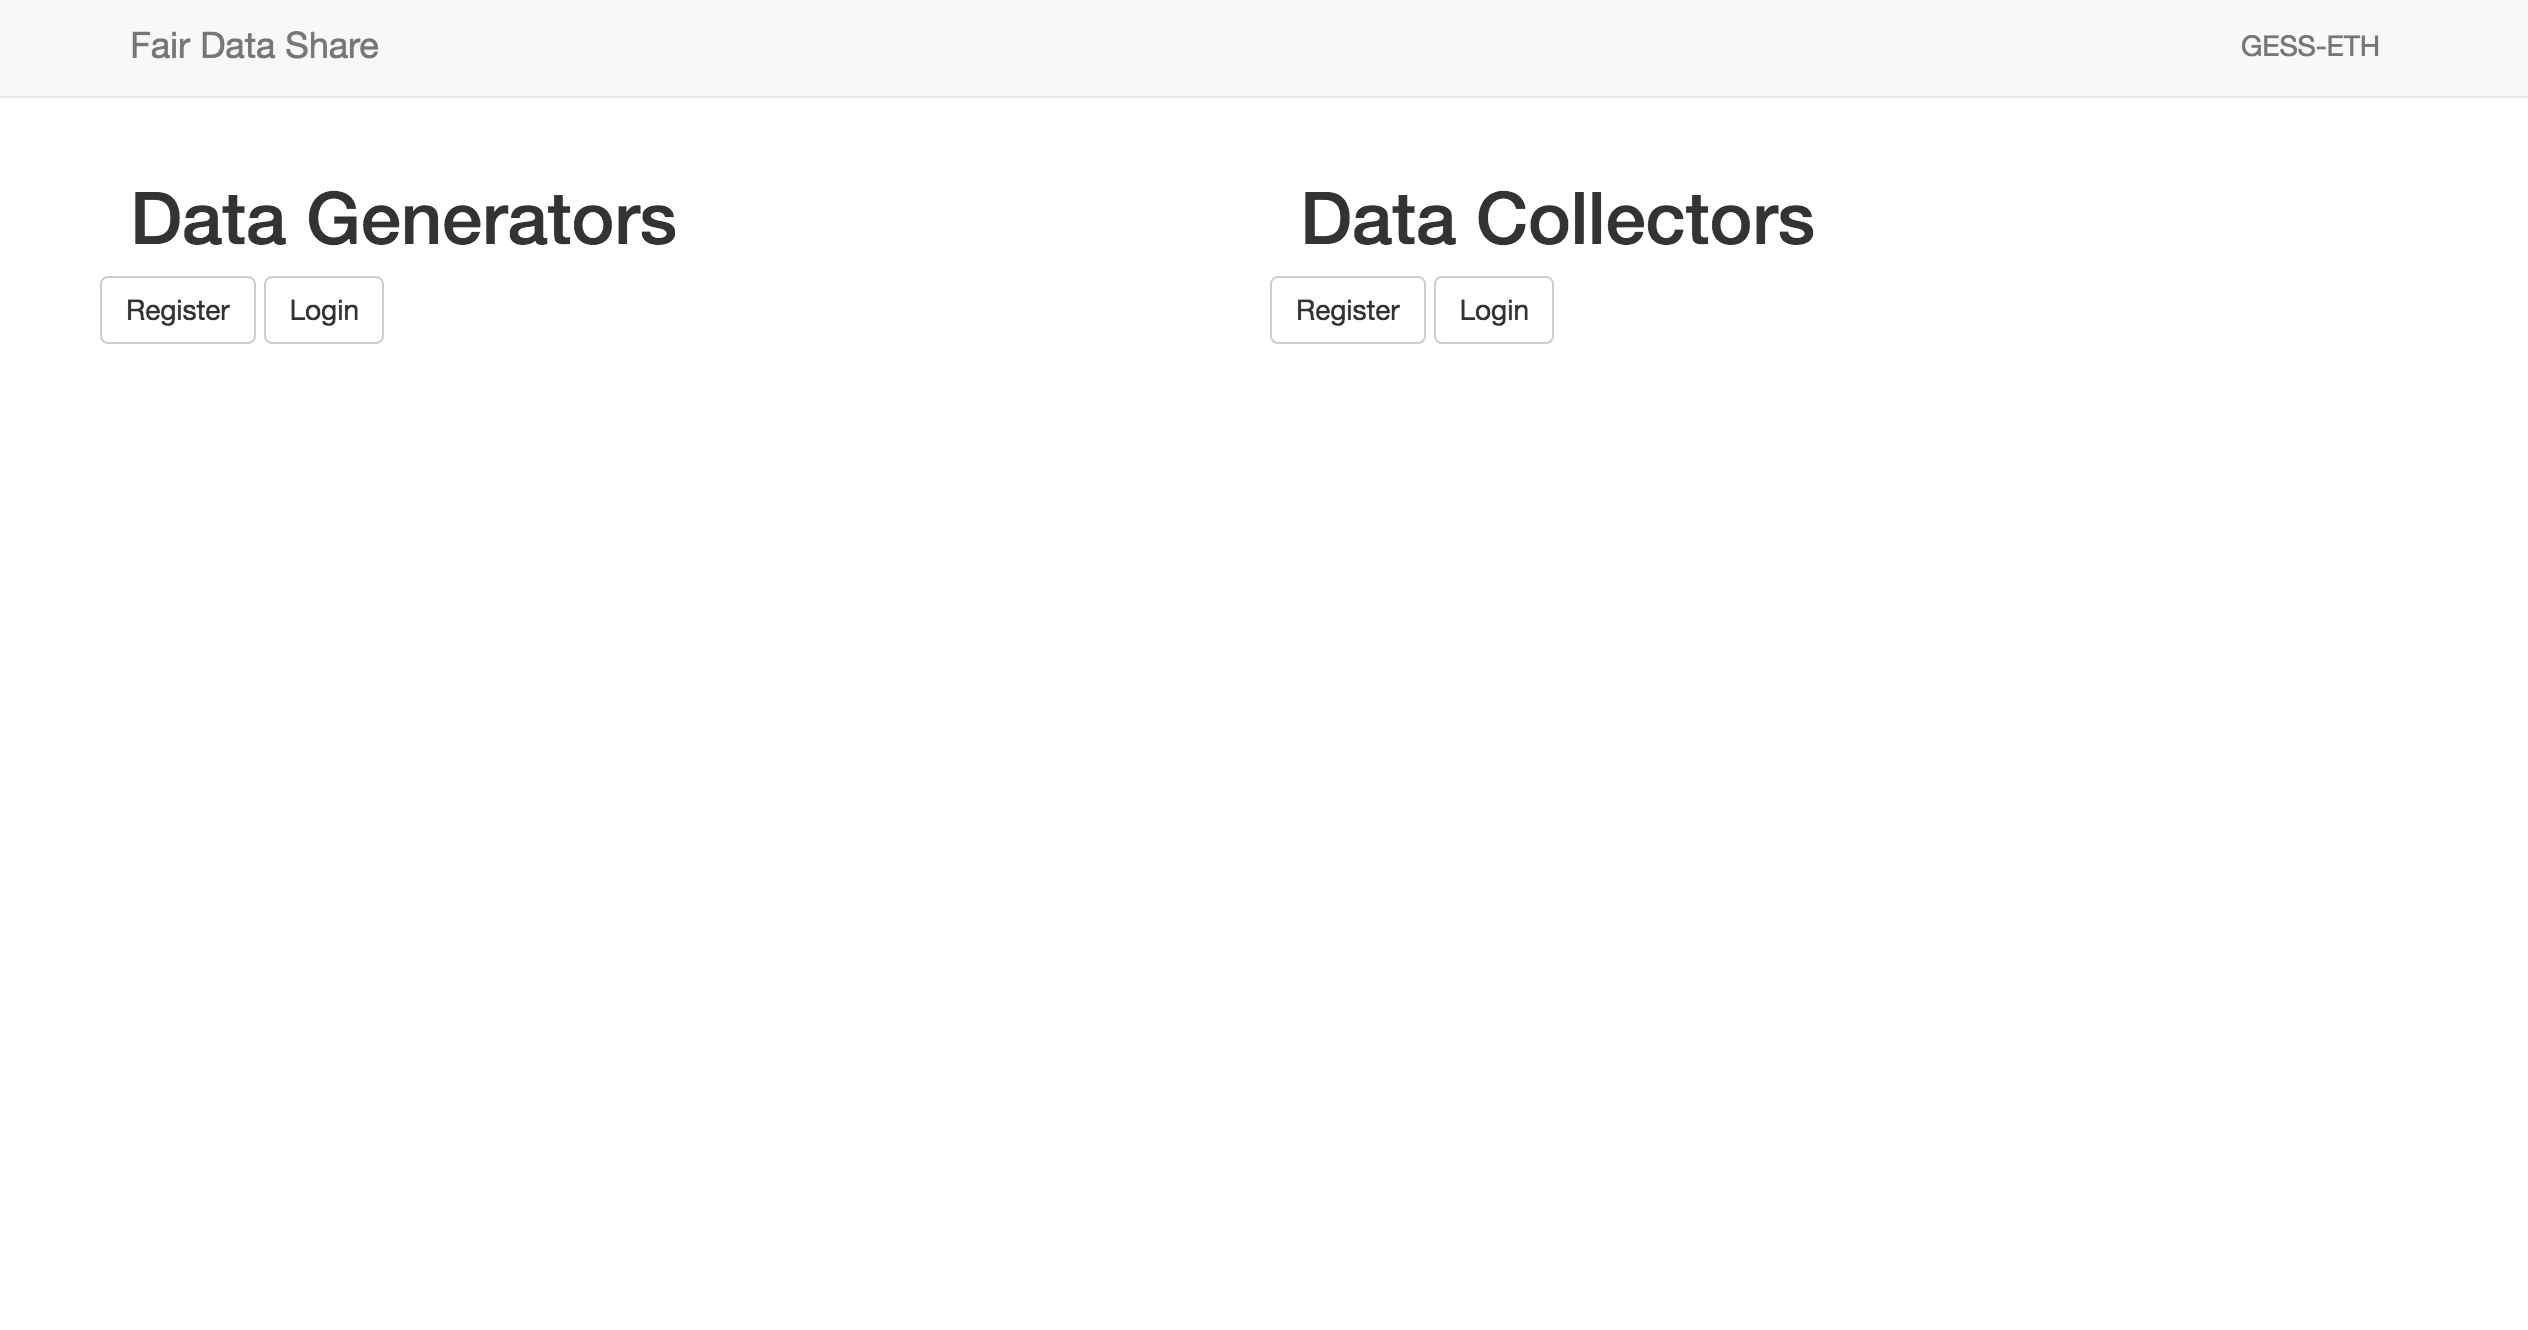
\includegraphics[width=\textwidth,keepaspectratio]{./images/fds}
\caption{FairDataShare Homepage}
\label{fig:fds_home}
\end{figure}

\begin{figure}[ht!]
\centering
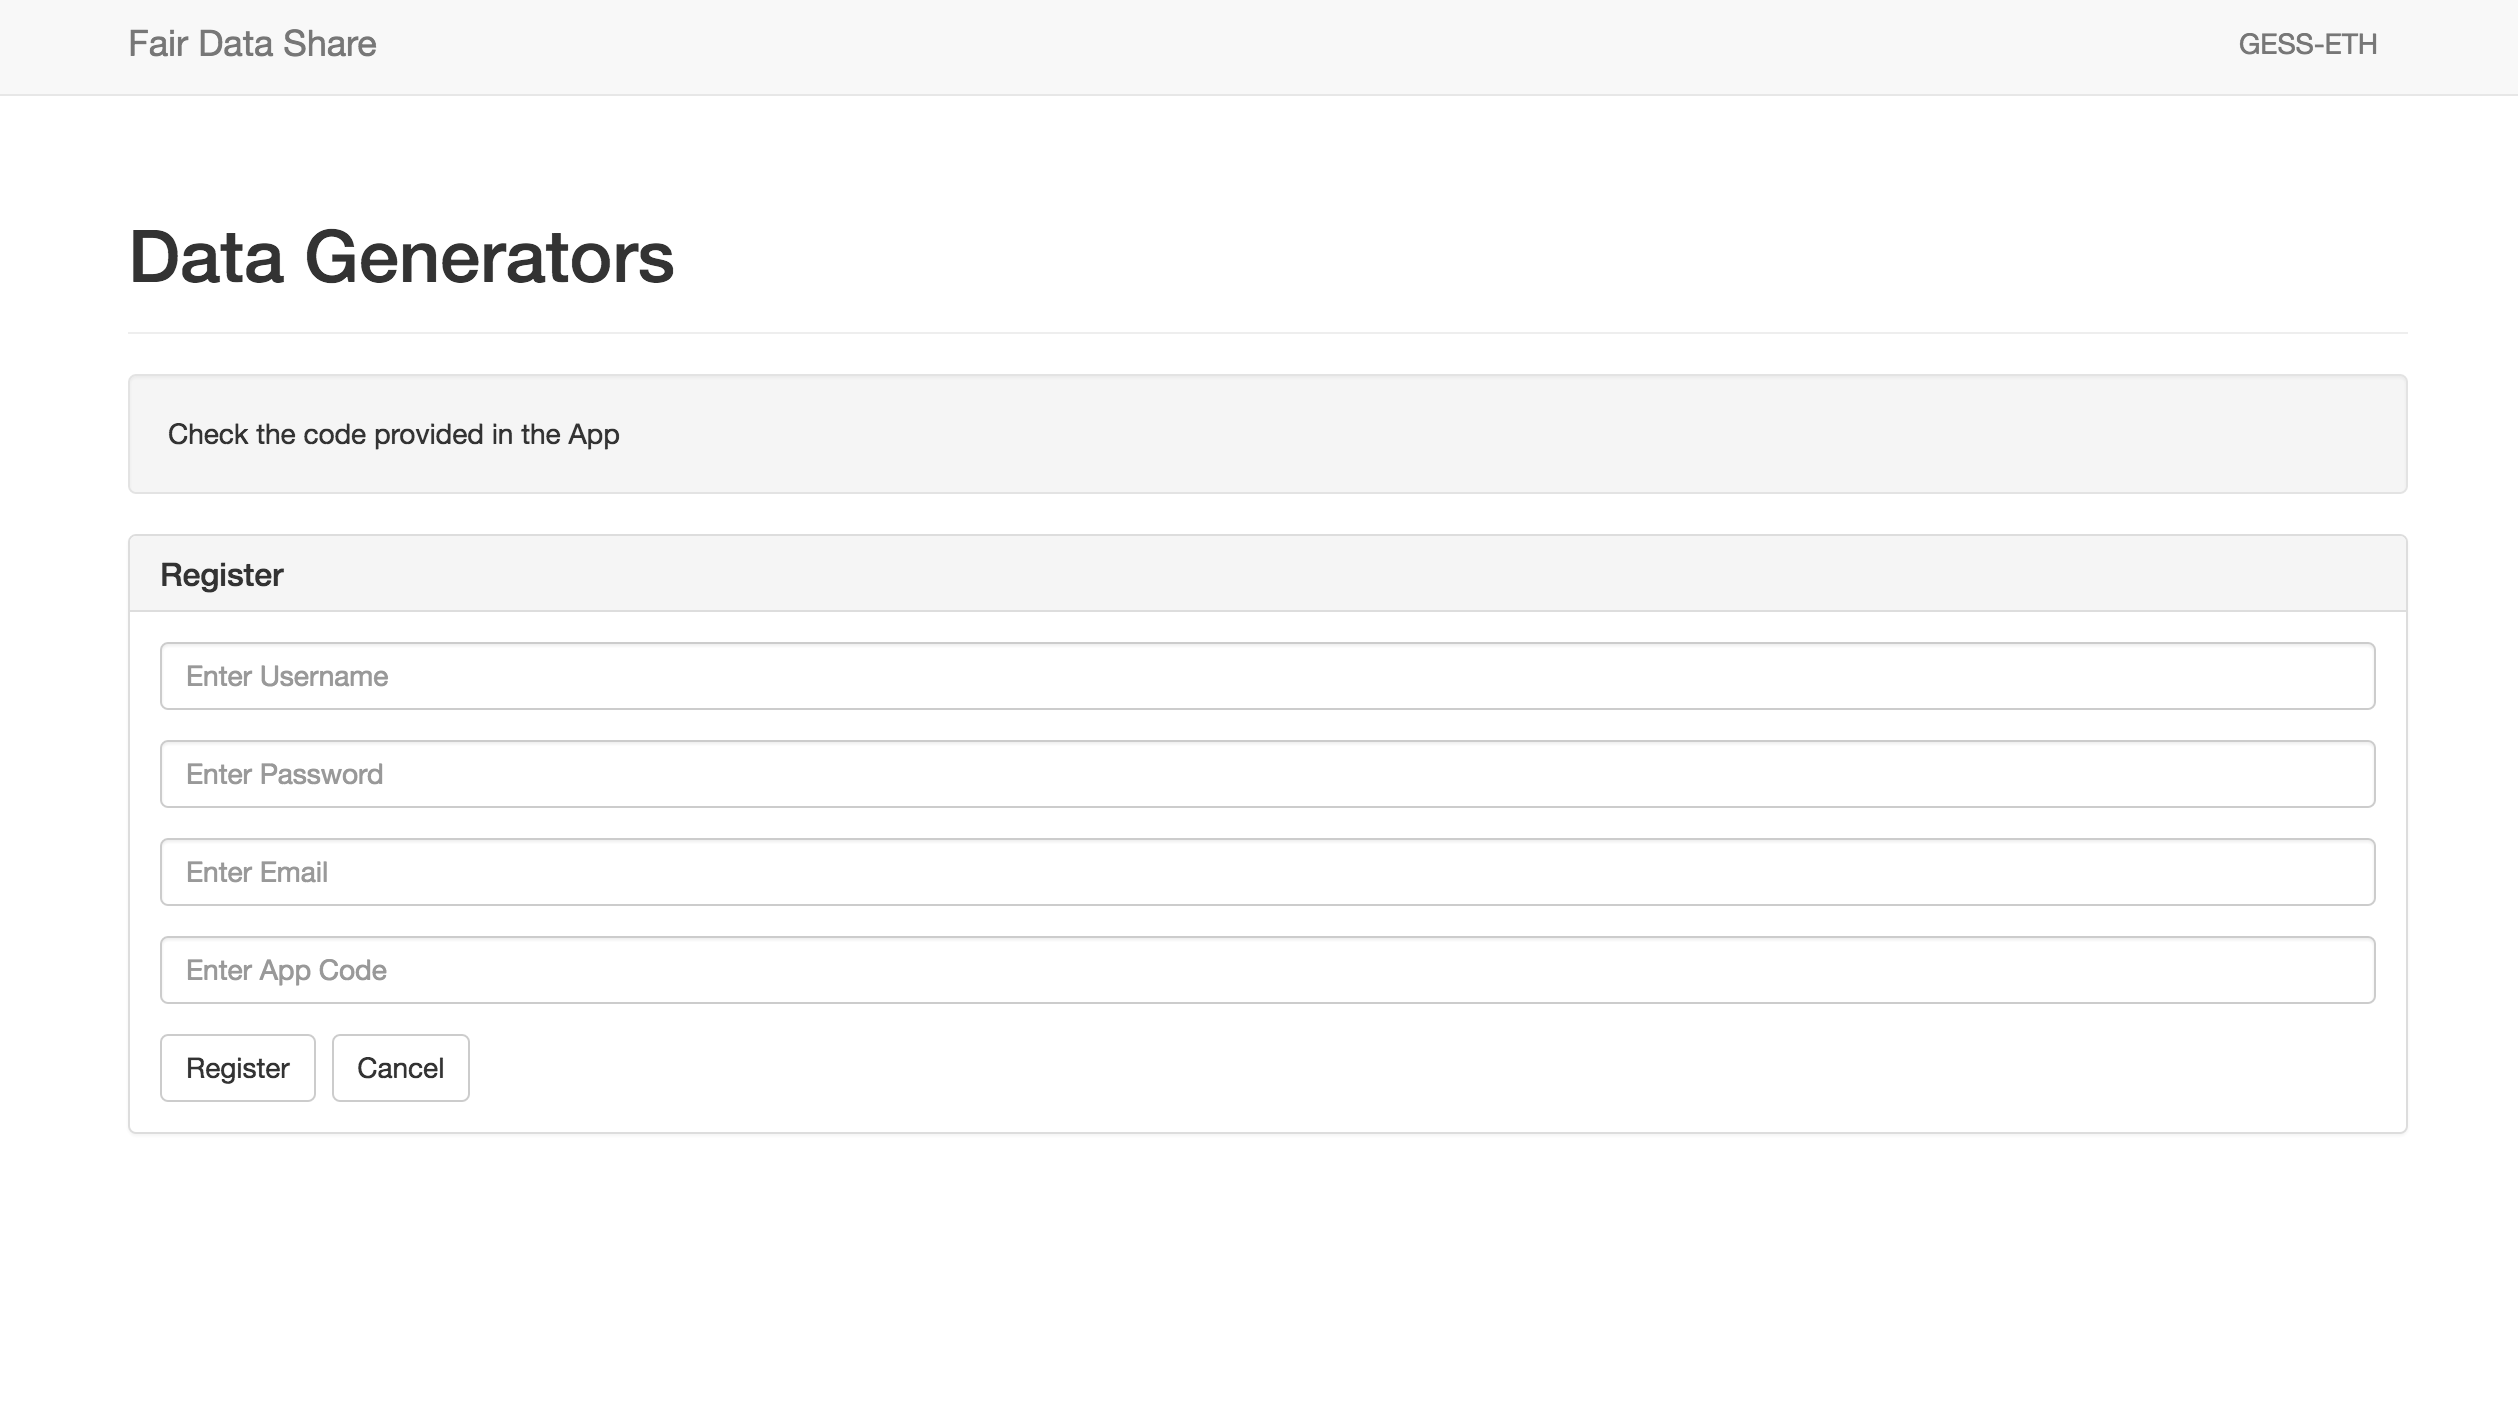
\includegraphics[width=\textwidth,keepaspectratio]{./images/fds_user_register}
\caption{Data Generators Registration Page}
\label{fig:first}
\end{figure}

The user can  login into the portal after a minimum of 24 hours after the start of the core phase to see the data that has been collected and shared with the stakeholders. 

In the task-bar, the user can see the bidding day number and how many questions have been answered from the total available shown by numbers 1 and 2 in the figure \ref{imp}. Day number one
corresponds to the day where users answer questions with no incentives of any kind and was presented in the previous sub-section. The screen presented after the entry phase is over is what is called the "improvement screen". 
The button numbered 3
represents "improve privacy" and the button numbered 4 represents "improve credit" respectively. The items numbered 6 and 5 represent the privacy percentage and credit obtained by the user respectively. Privacy is measured in terms of the percentage of mobile sensor data not traded to the stakeholders. Credit is measured in terms of the currency Swiss Francs obtained for trading data to the stakeholders. 

The item numbered 7 is the round number which indicates the number of times the user has answered all the data requests. The item numbered 2 is the number of questions the user has answered in the current round. Item number 1 indicates the experiment day number.



\begin{figure}[htp]
  \subtop[Bidding Screen\label{fig:bid1}]{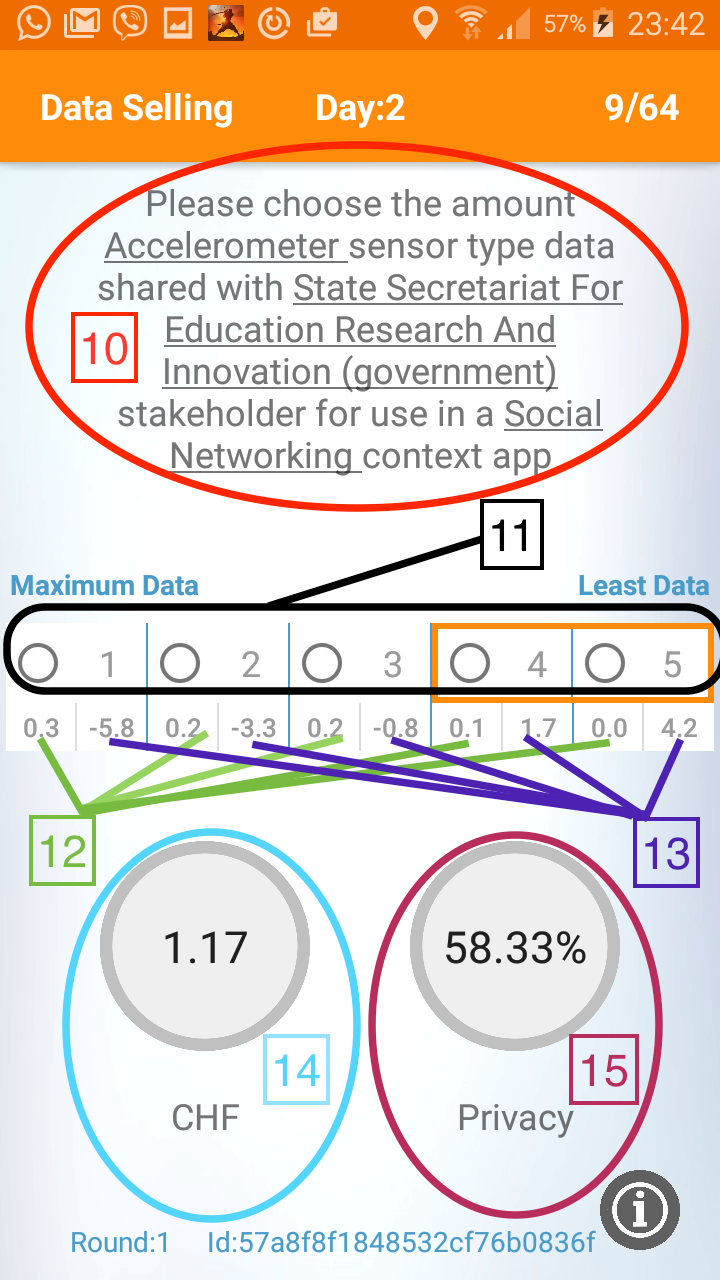
\includegraphics[width=0.4\linewidth]{./images/bid_layout_1}}\hspace{1em}
  \subtop[Bidding Screen with Submit Button \label{fig:bid2}]{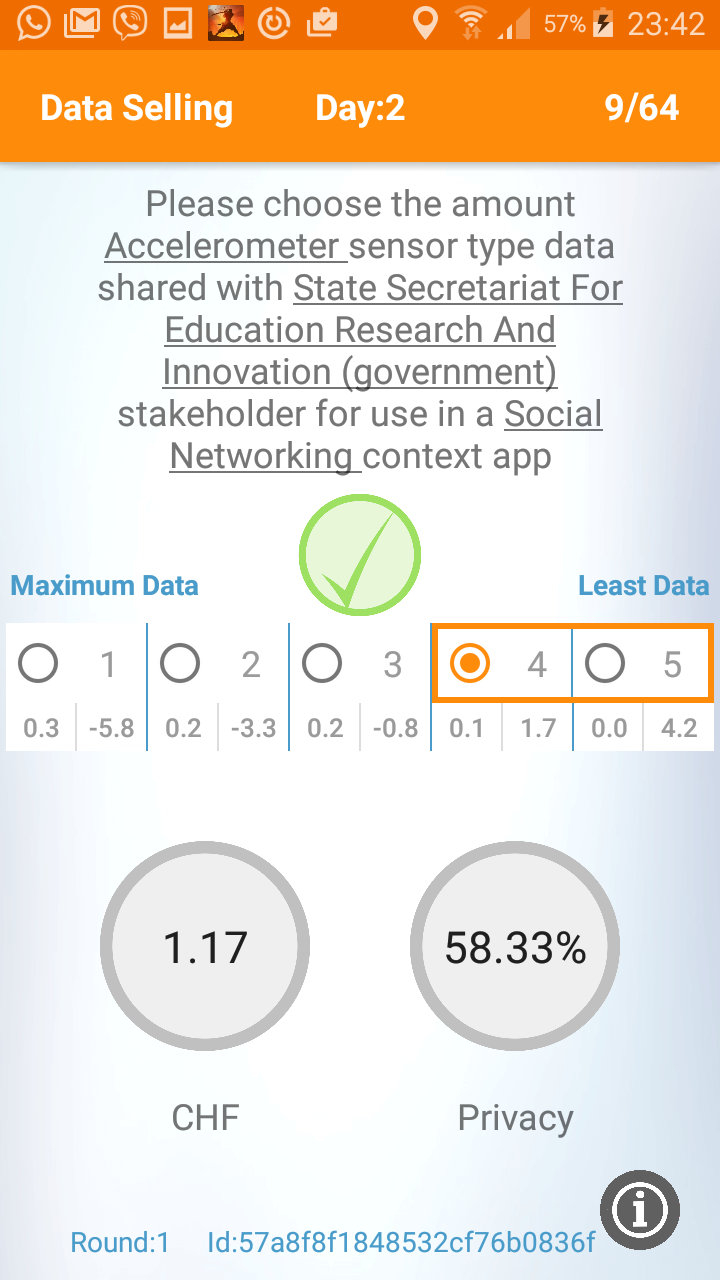
\includegraphics[width=0.4\linewidth]{./images/bid_layout_2}}%
  \caption{FairDataShare Portal}
  \label{fig:bid}
\end{figure}


There are a total of 64 data requests, hence after all the 64 have been answered, the number of questions answered is reset and the number of rounds answered increases by one. This indicates all the data requests that have been answered and how many are left unanswered. Each question will have 5 options to choose from, ranging from maximum data sharing to least data sharing.

From the starting time of the core phase till 24 hours later marks one bidding day. Once 24 hours is over, another bidding day starts where the privacy and credit metrics are reset. The day number in the task bar is incremented by one. The user has to answer all the data requests again for this new bidding day. Previous responses to data requests are not carried over to the next day. If a data requests is not answered, it is considered that the user does not want to trade mobile sensor data for that request. Additionally, each data request carries a participation fee, this is irrespective of the amount of mobile sensor data shared, by not participating in a data request the user foregoes this credit gain.
The core phase goes on for a period of 48 hours. 

\subsection{Improve Privacy or Credit}

The improvement screen shown in figure \ref{fig:imp} is where users can choose whether they would like to improve the privacy or the credit. The elements of this screen have been explained in the previous section \ref{core}.
The improve credit button
should be chosen if the user is interested in maximizing the amount of credit obtainable. This uses an algorithm that uses the previous user answers to
put forth a data request that can increase the credit to the maximum explained in section \ref{data_req}. The credit improvement button is represented by the item number 5. Similarly, the improve privacy button is used to further improve the privacy that has been obtained. This puts forth a data request that can further increase the user privacy. It needs to be noted that the ultimate change in the privacy or credit metrics depends on the option chosen by the user for the data request. The privacy improvement button is represented by the number 6.

Scenario examples for each button is given in the next section after introducing the next screen in the application. For example, if a user chooses to improve the privacy, then clicks on improve privacy button and gets a data request. The user still chooses option one with maximum data sharing (least privacy) for the data request, this may not improve his privacy but decrease it. This is because option 1 indicates that the user trades all the data for this request without filtering the sensor information. Trading all data gives the user more credit, but decreases the privacy metric.

Similarly, if a user chooses to improve the credit obtainable, the user clicks on the improve credit button and gets a data request. Then the user chooses the option five with least data sharing (maximum privacy) which indicates that no data is traded for this request. This response counters the initial desire to improve the credit obtainable. Trading no data increases one's privacy, but does not increase the credit to the maximum. Therefore, an actual improvement in the chosen metric depends on the chosen improvement button chosen and the choice of the appropriate option for that data request.

\subsection{Answering Questions with Incentives}

After choosing a metric to improve, a screen is presented as shown in figure \ref{fig:bid1}.
This screen is called the "bidding screen". This screen is very similar to the screen \ref{fig:imp} presented in the entry phase, except that the user
is aware of the amount of privacy and credit obtained as indicated by items 14 and 15 respectively. Additionally, the user can see information about how the privacy and credit will increase or decrease for each privacy option of a data request. The items numbered 11 are the privacy options ranging from one to five.

The items numbered 12 are the improvement in privacy for each possible option of the current data request shown as item numbered 10. The items numbered 13 are the improvements in credit for each possible options of the current data request. Once the user decides on which options to choose according to how much data wants to be traded, the users can click on the radio option as explained in section \ref{options} and then click again on the green submit button that pops up shown in \ref{fig:bid2} to confirm the answer. Once the green button has been clicked on, answers cannot be changed. The user has the possibility to go back to the improve screen from the bidding screen using the back button. Using the back button in the improve screen leads the user out of the application.

\begin{figure}[htp]
  \subtop[Example 1\label{fig:orange1}]{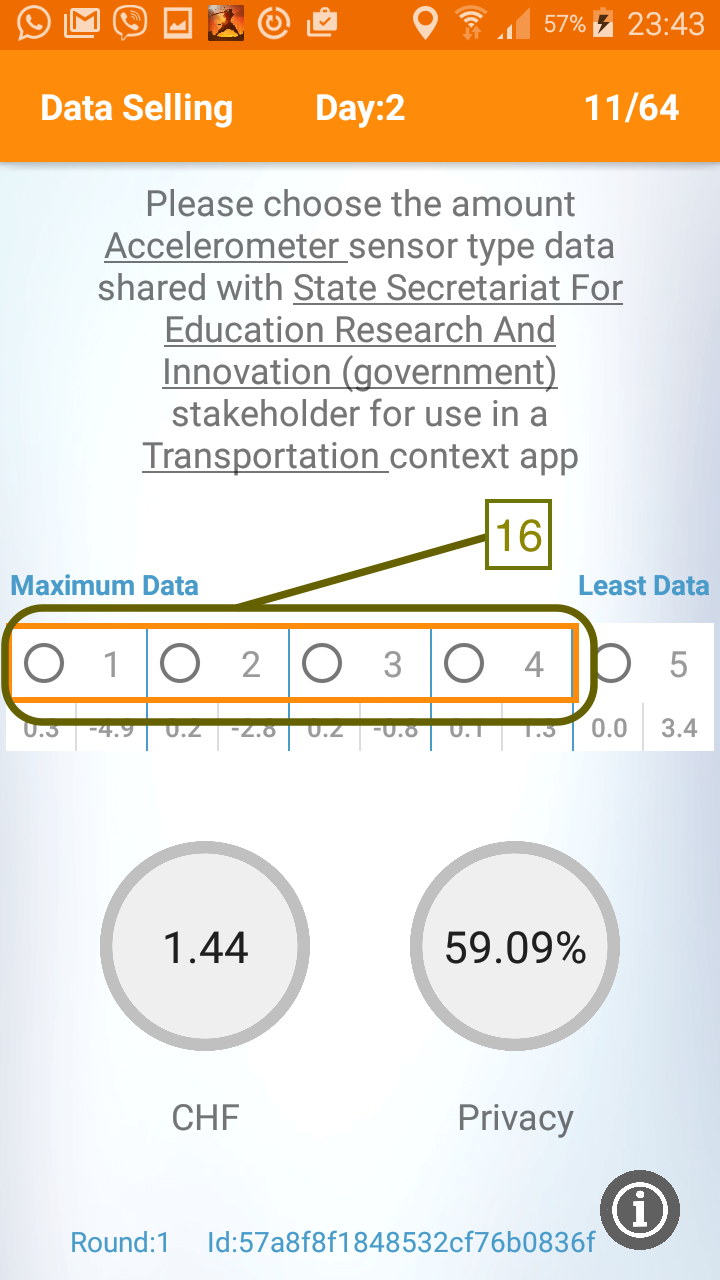
\includegraphics[width=0.4\linewidth]{./images/bid_layout_3}}\hspace{1em}
  \subtop[Example 2 \label{fig:orange2}]{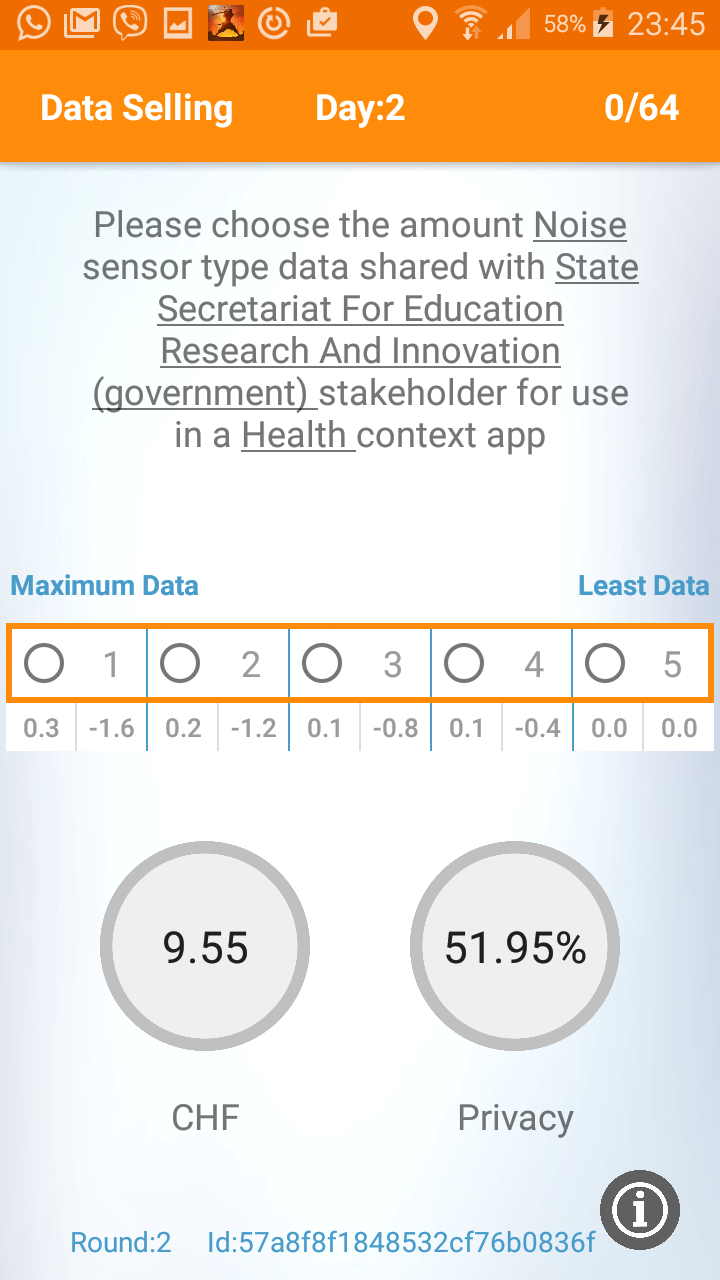
\includegraphics[width=0.4\linewidth]{./images/bid_layout_5}}%
  \caption{Recommendation Box}
  \label{fig:orange}
\end{figure}

Additionally, for every question there is an orange recommendation box surrounding some options. This recommendation is highlighted by the number 16 in figure \ref{fig:orange1}.
This gives an indication to the user as to which options can improve the privacy or the credit compared to the previous time the user has
answered this data request. For example, if the user has previously answered option 4 to a data request and has clicked on improve credit, the system
puts an orange box around options 1,2,3 and 4. Similarly, if the user clicked on improve privacy button, and the users previous answer was option 1, the system would recommend the options 1,2,3,4 and 5. Two examples of this are provided in figures \ref{fig:orange}. 

It needs to be noted that the orange box does not necessarily provide an improvement of the particular metric chosen, it is meant to indicate improvements compared to the previous time the data request was answered to.


\section{Exit Phase}

After the end of the core phase, the participants are asked to fill up a survey based on their experience in the experiment. Some questions are
about the rewards received, the privacy and credit metrics, design of the application, and how the experiment was conducted. The survey \footnote{\url{https://descil.eu.qualtrics.com/SE/?SID=SV_3P0ySMqNeOO6v5j}} is linked to the user using the unique identifier assigned in the application. Once the survey is filled, the users receive their money for the entry phase, core phase and exit phase together, but only if they did not have their phones switched off throughout the experiment and participated in the core phase. This is done by checking the data collected on the server.

\section{FairDataShare Web Portal} \label{fds}

The FairDataShare portal \footnote{\url{http://fair-data-share.inn.ac/}} is a website where users can view the data collected from them during the core phase of the experiment. Below is an explanation of how users and stakeholders can view mobile sensor data.

\subsection{Data Generator's Portal}

Once the users are registered which was explained in section \ref{core}, they can come back to the portal after a 24 hours period or later to view their mobile sensor data collected in the server. The data portal login page is shown in figure \ref{fig:fdslogin}. Since the users are already registered from the mobile phone in the entry phase, they can go to the portal from their computers and this time login instead of register. Users should enter their: 

\begin{enumerate}
    \item Username
    \item Password
\end{enumerate}

Once this is done, users will be redirected to the data collection page shown in figure \ref{fig:fdsdash} with the following options in the task-bar  to choose from:

\begin{enumerate}
    \item Accelerometer
    \item Light
    \item Noise
    \item Location
\end{enumerate}

Users can choose the sensor from the task-bar whose data they want to see by clicking on it. The data displayed includes the following columns :

\begin{enumerate}
    \item Timestamp
    \item Bidding day
    \item Sensor Values
\end{enumerate}

Figures \ref{fig:fdsgps}, \ref{fig:fdslight}, \ref{fig:fdsacc} and \ref{fig:fdsnoise} show examples of the data that can be seen for the location,
light, accelerometer and noise sensor.



\begin{figure}[htp]
  \subtop[Login Page\label{fig:fdslogin}]{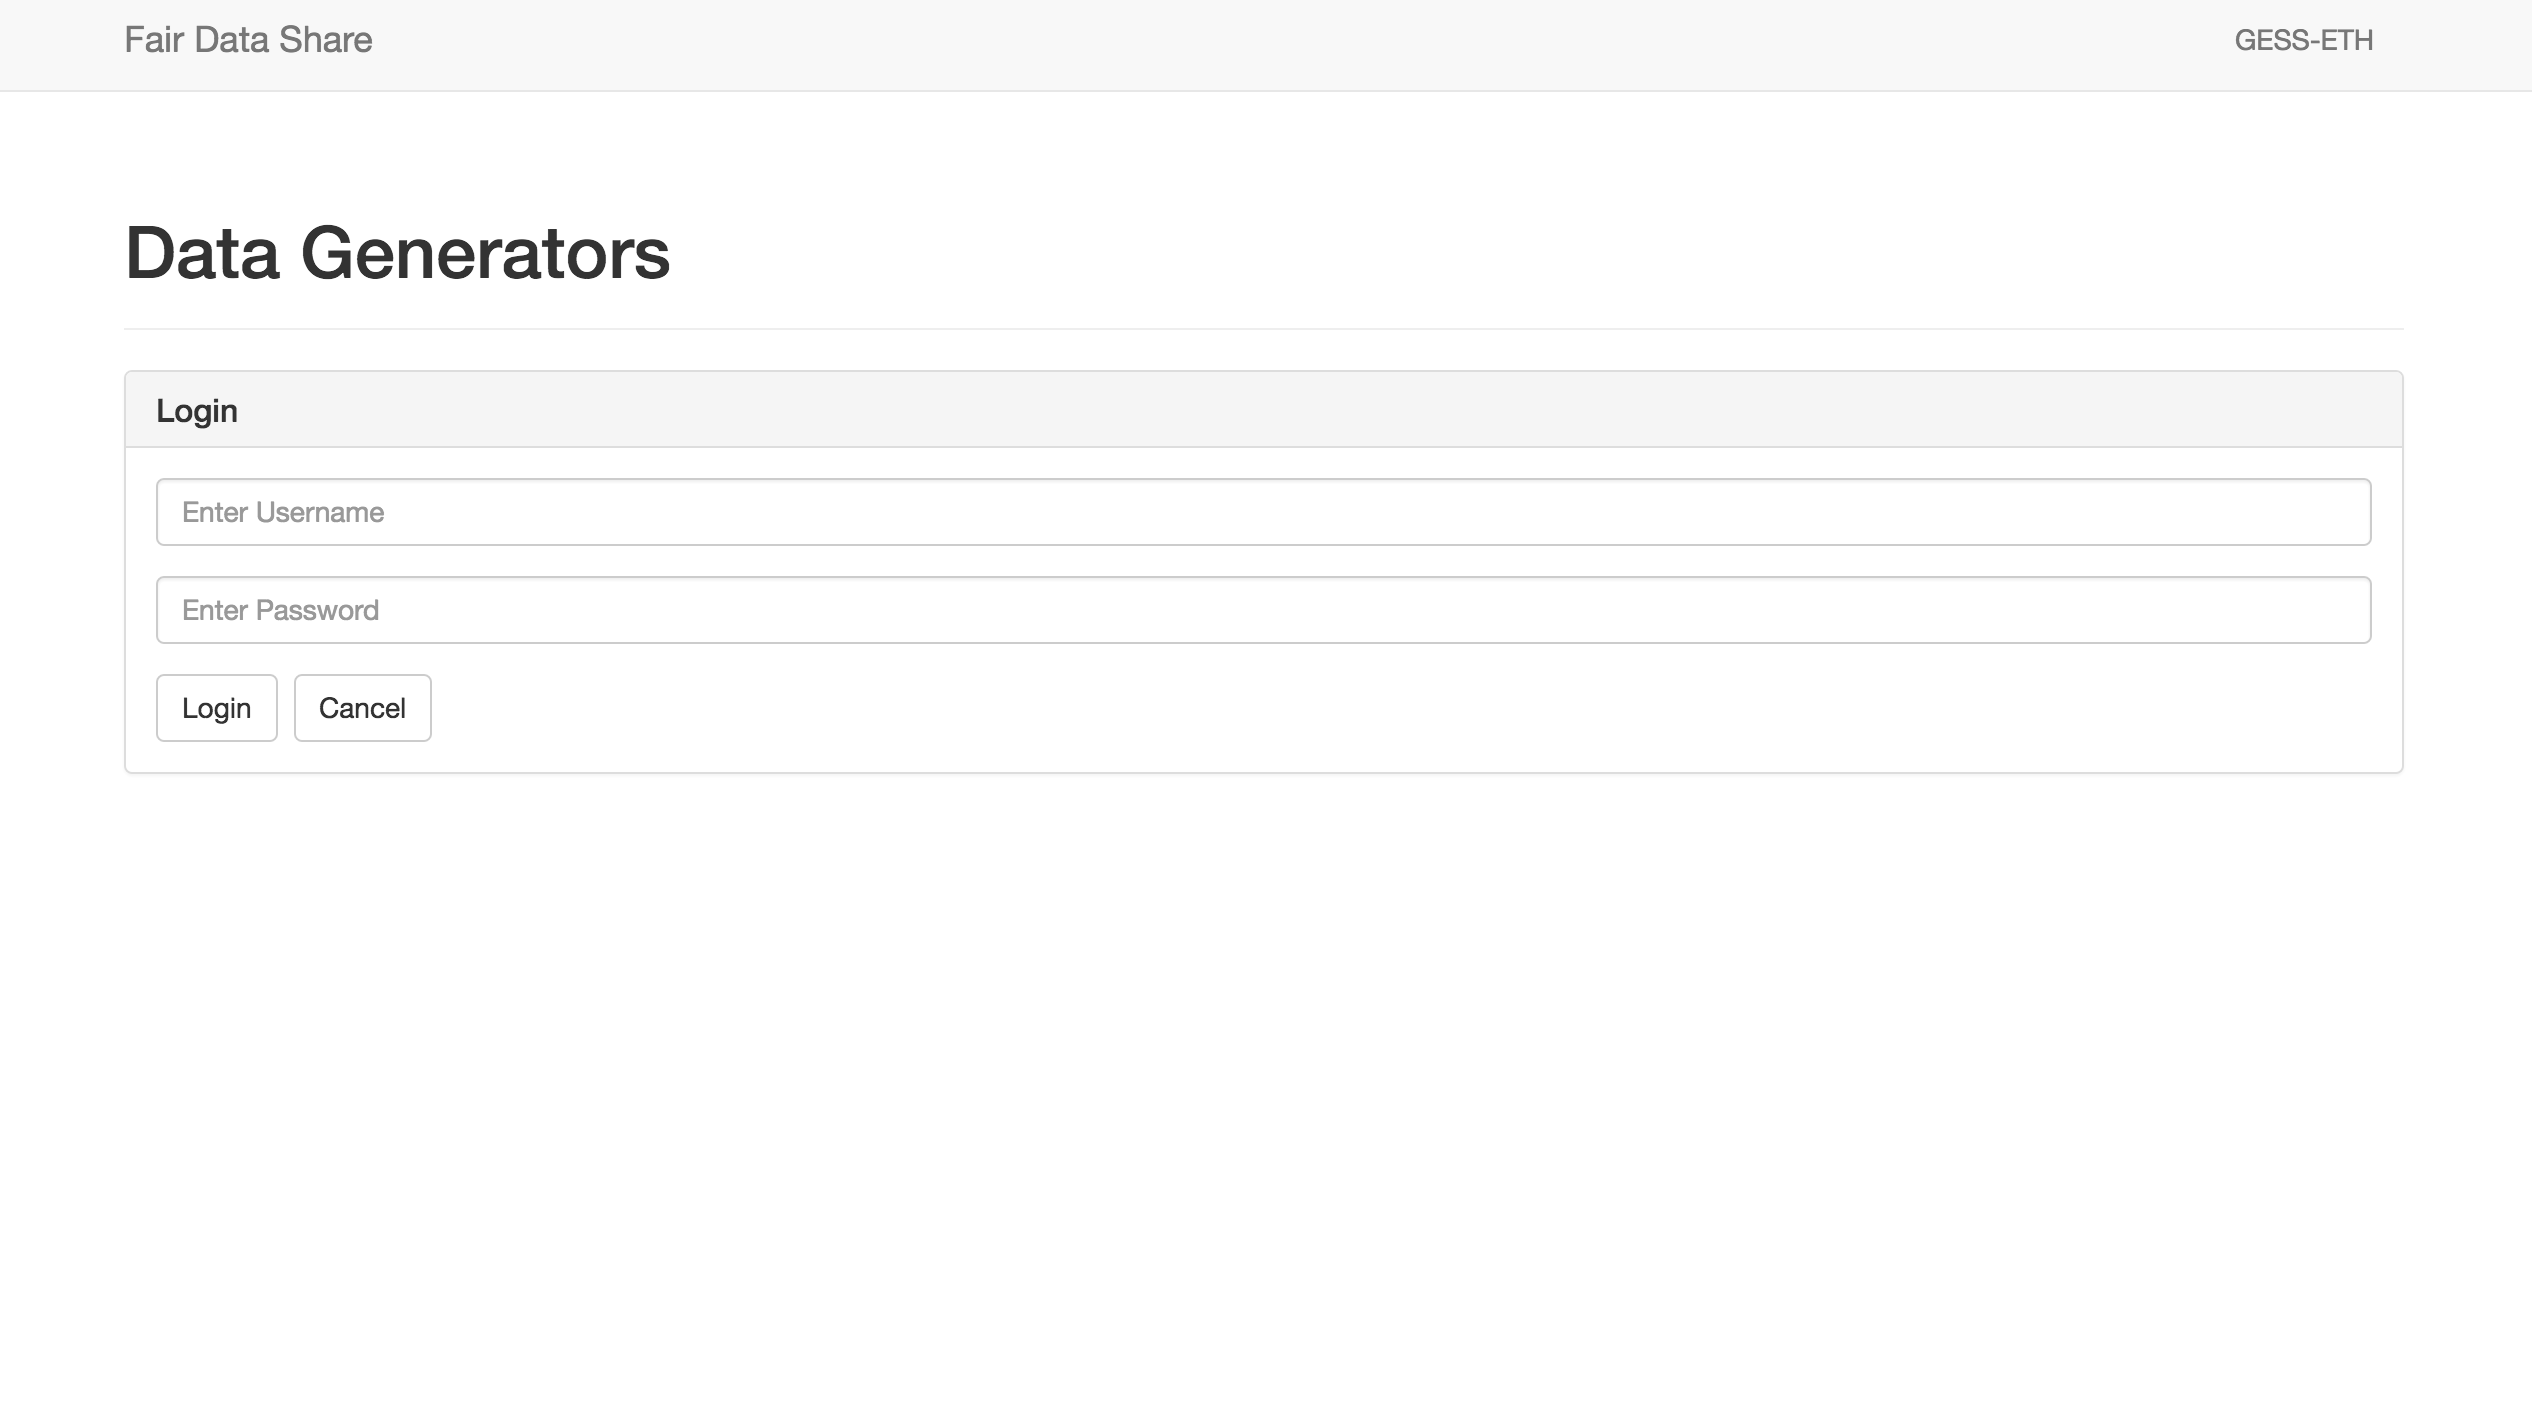
\includegraphics[width=0.4\linewidth]{./images/fds_user_login}}\hspace{1em}\hspace{1em}
  \subtop[ Welcome Page\label{fig:fdsdash}]{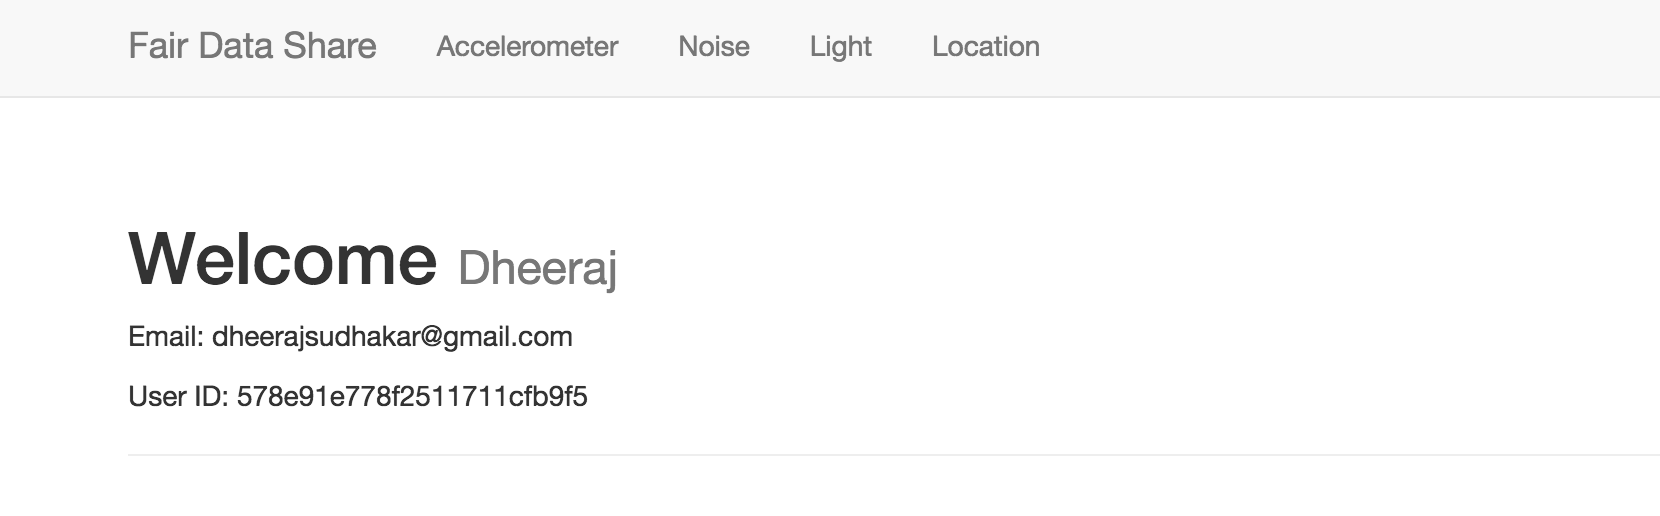
\includegraphics[width=0.4\linewidth]{./images/fds_user_welcome}}%
  \caption{Entering the Portal}
  \label{fig:fds1}
\end{figure}

Users first register as data generators as indicated in the section \ref{quest_wi}.
\begin{figure}[htp]
  \subtop[Location Data\label{fig:fdsgps}]{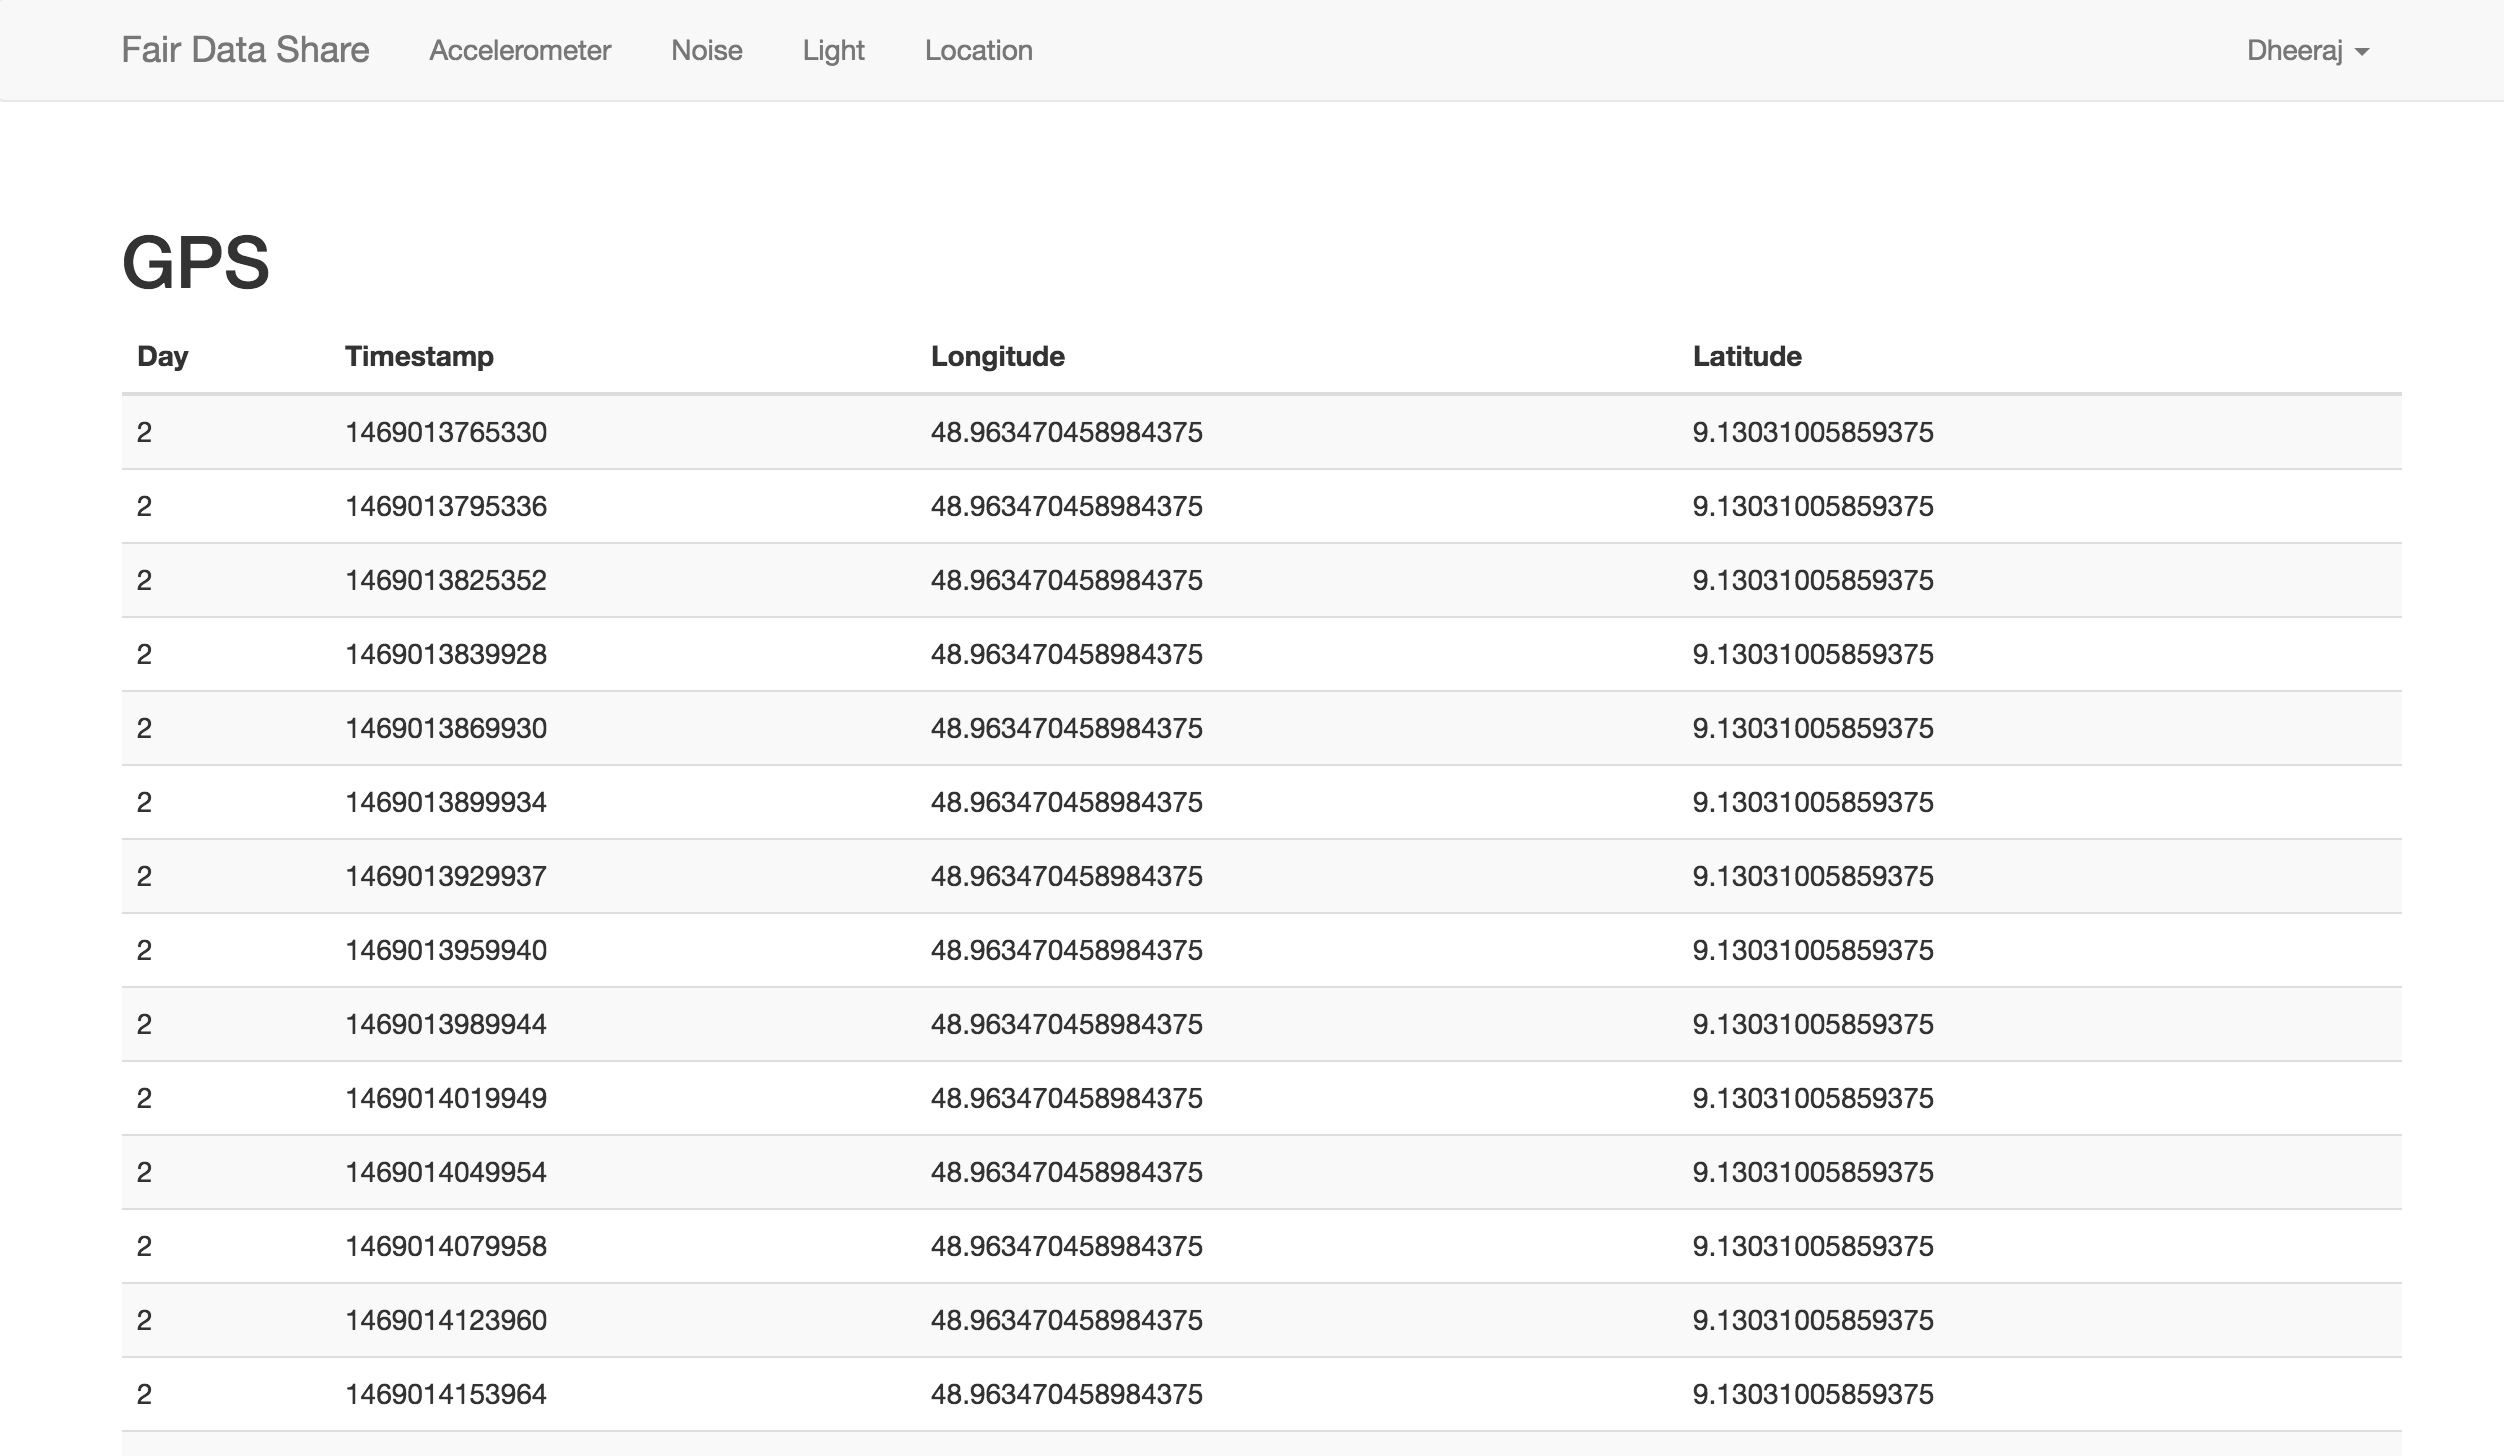
\includegraphics[width=0.4\linewidth]{./images/fds_user_gps_full}}\hspace{1em}\hspace{1em}
  \subtop[Light Data \label{fig:fdslight}]{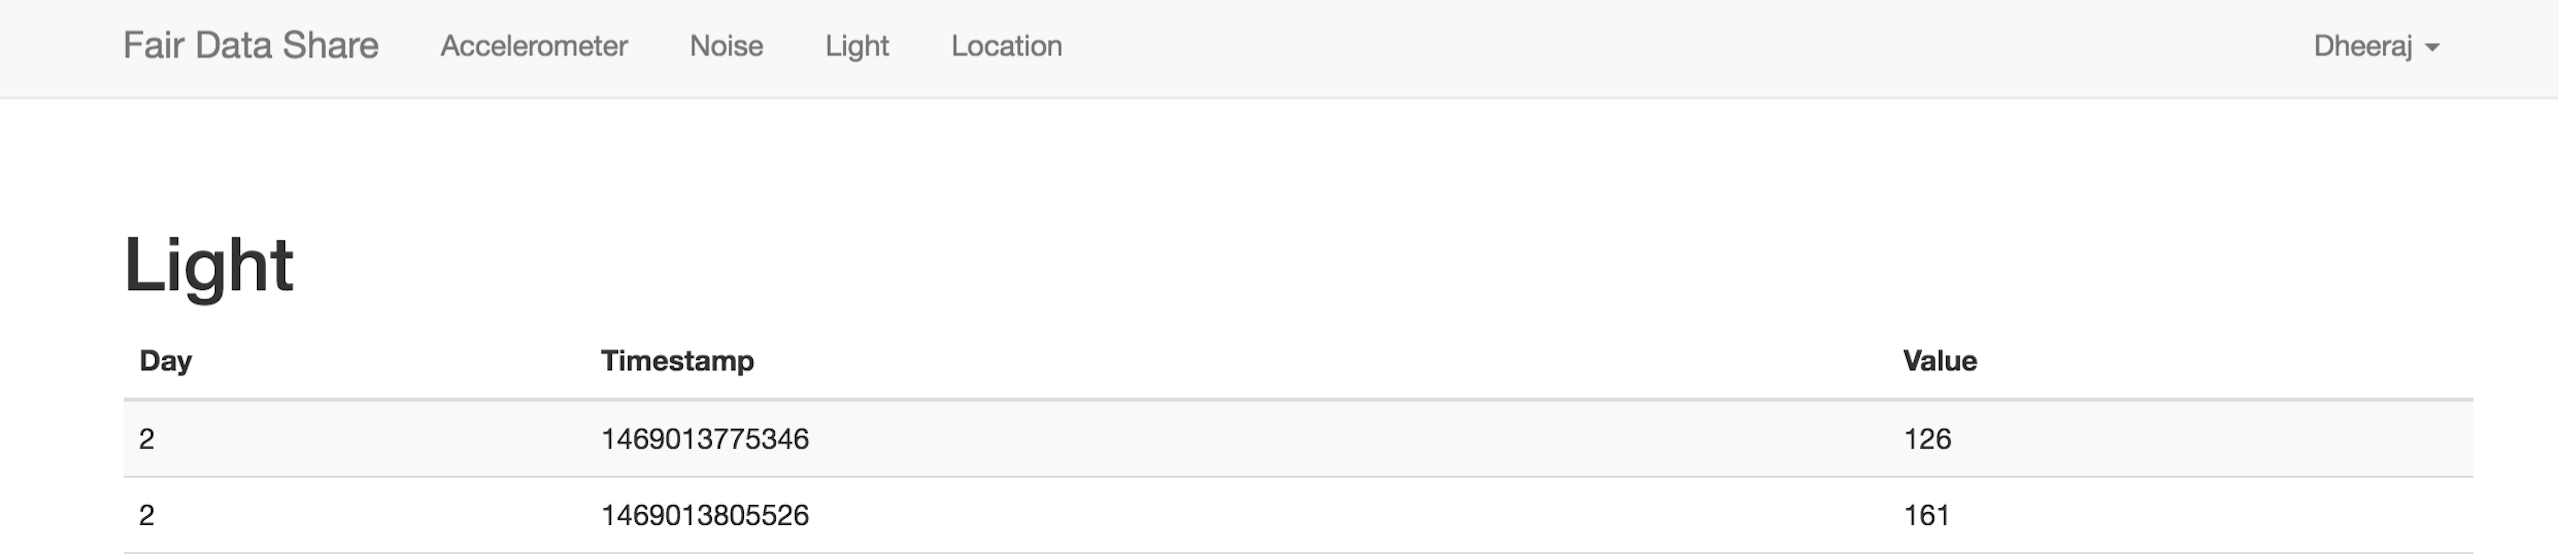
\includegraphics[width=0.4\linewidth]{./images/fds_user_light_full}}%
  \caption{User Data}
  \label{fig:fds2}
\end{figure}

\begin{figure}[htp]
  \subtop[Accelerometer Data\label{fig:fdsacc}]{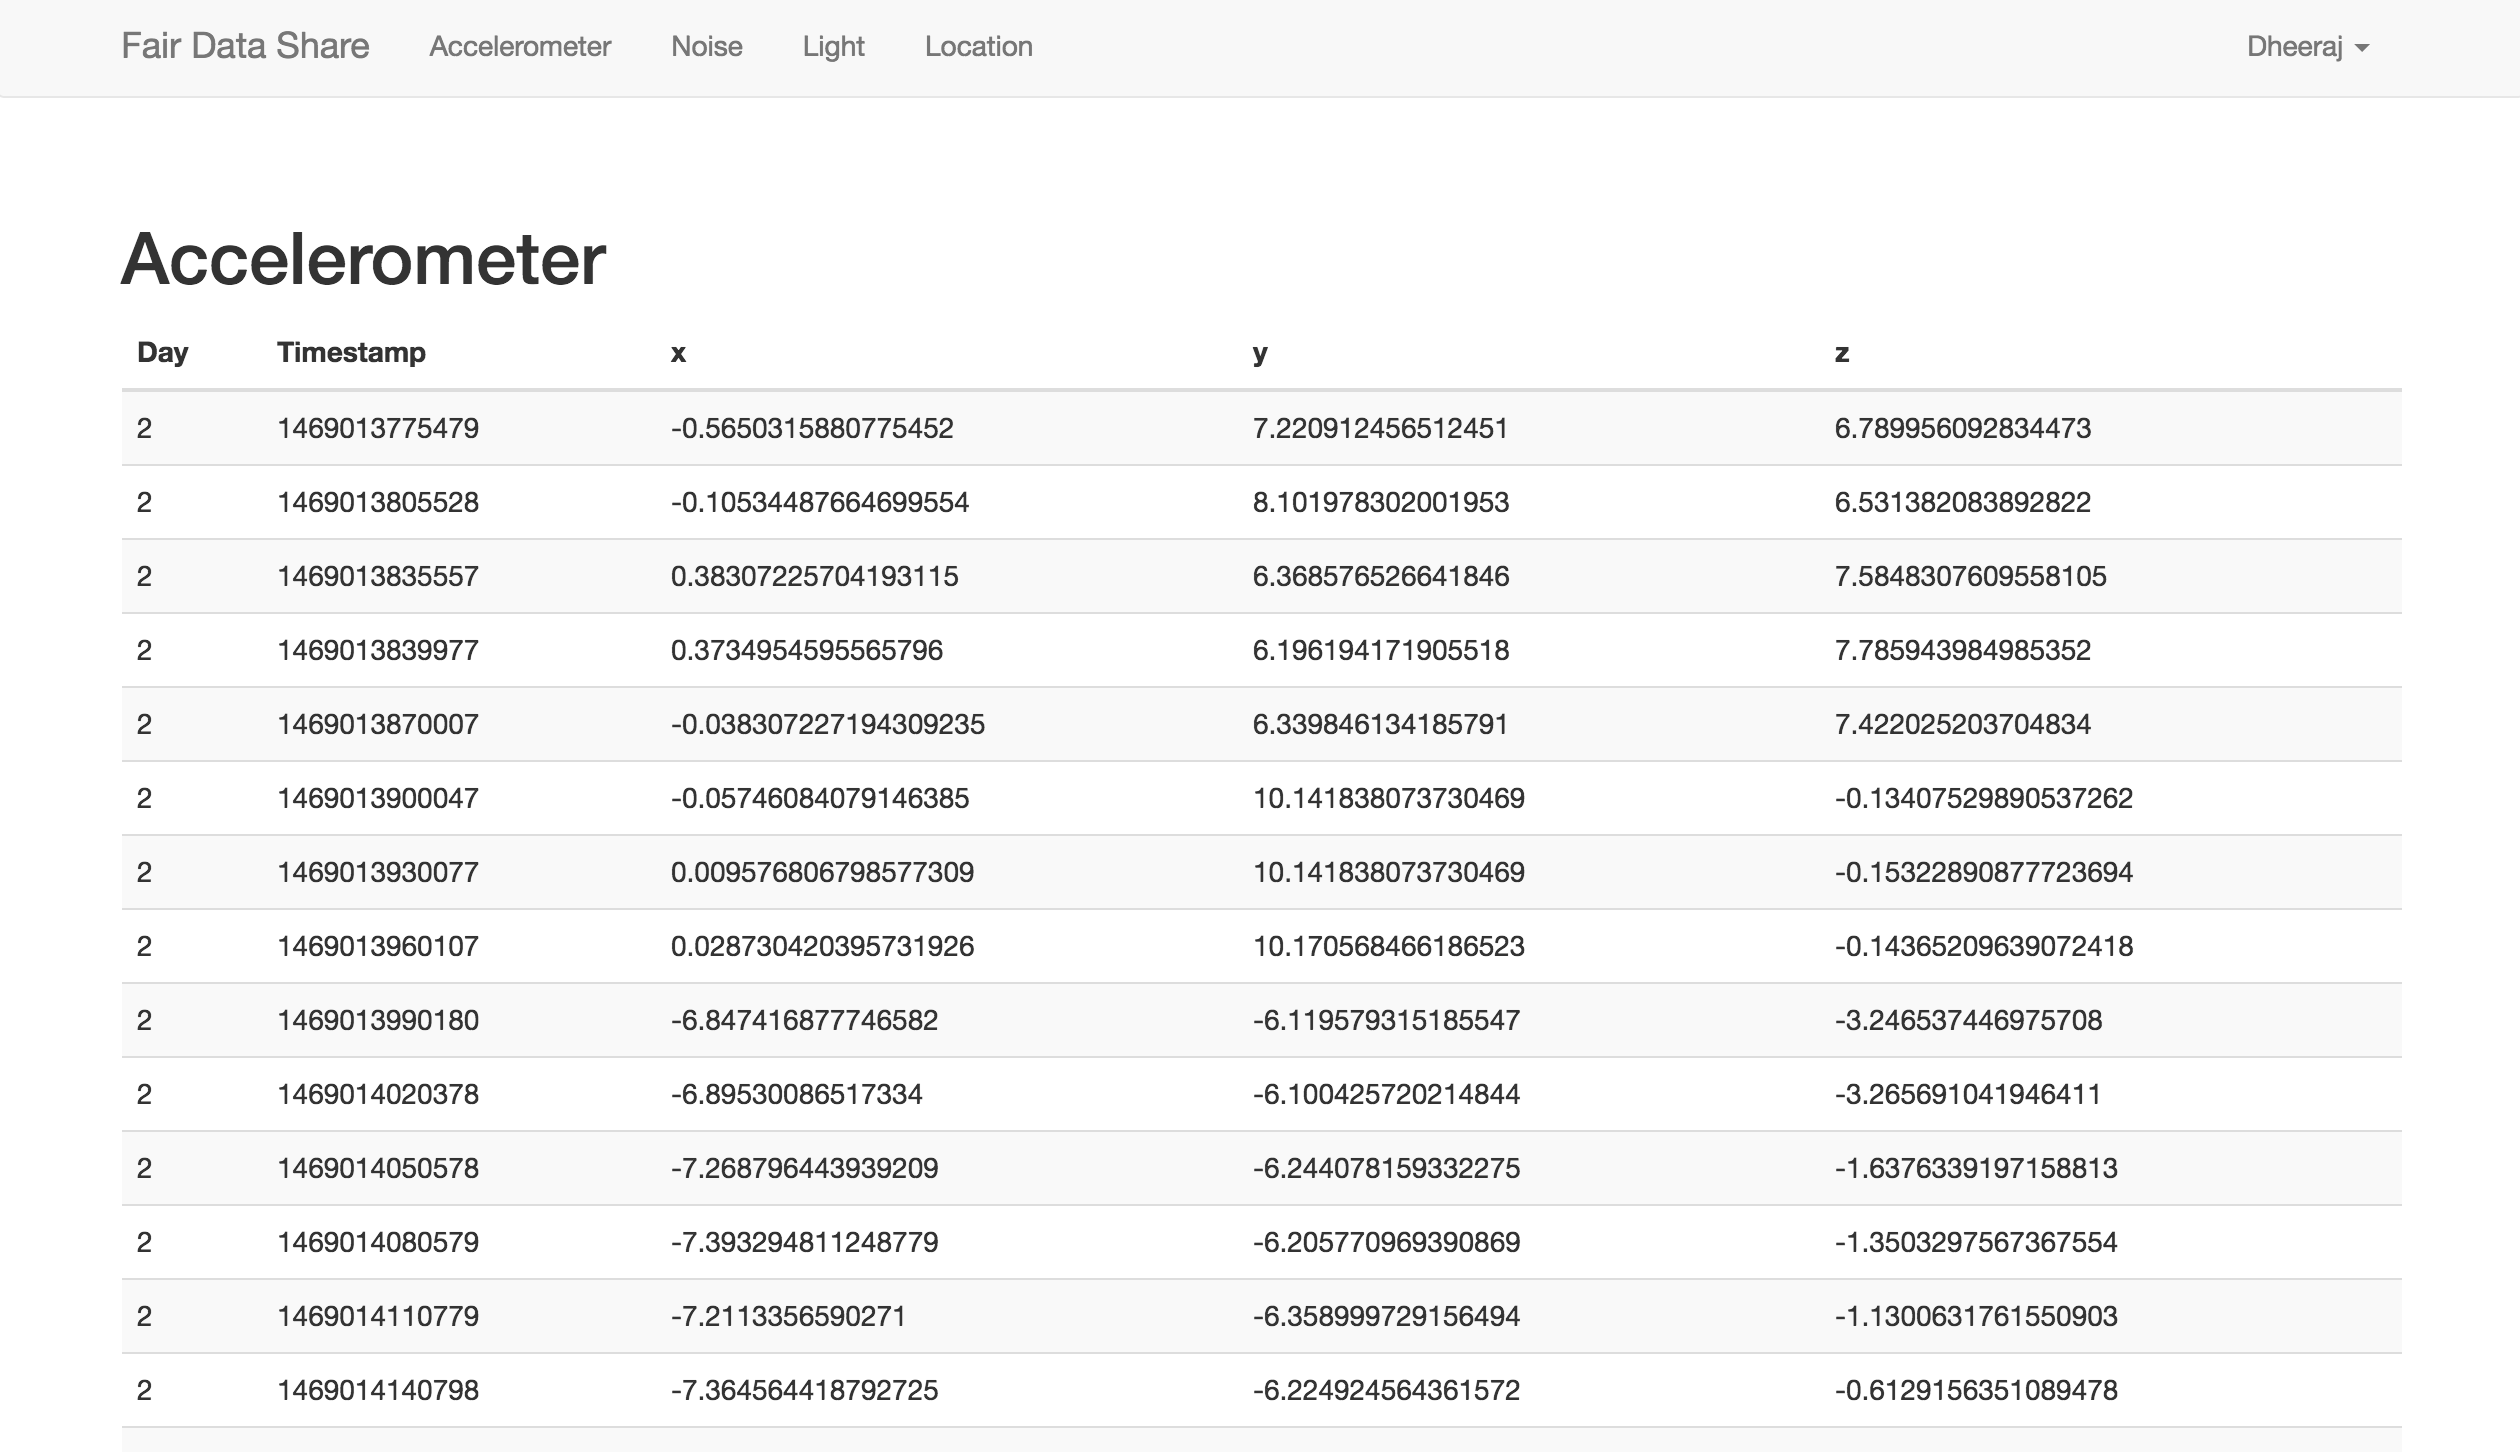
\includegraphics[width=0.4\linewidth]{./images/fds_user_acc_full}}\hspace{1em}\hspace{1em}
  \subtop[Noise Data \label{fig:fdsnoise}]{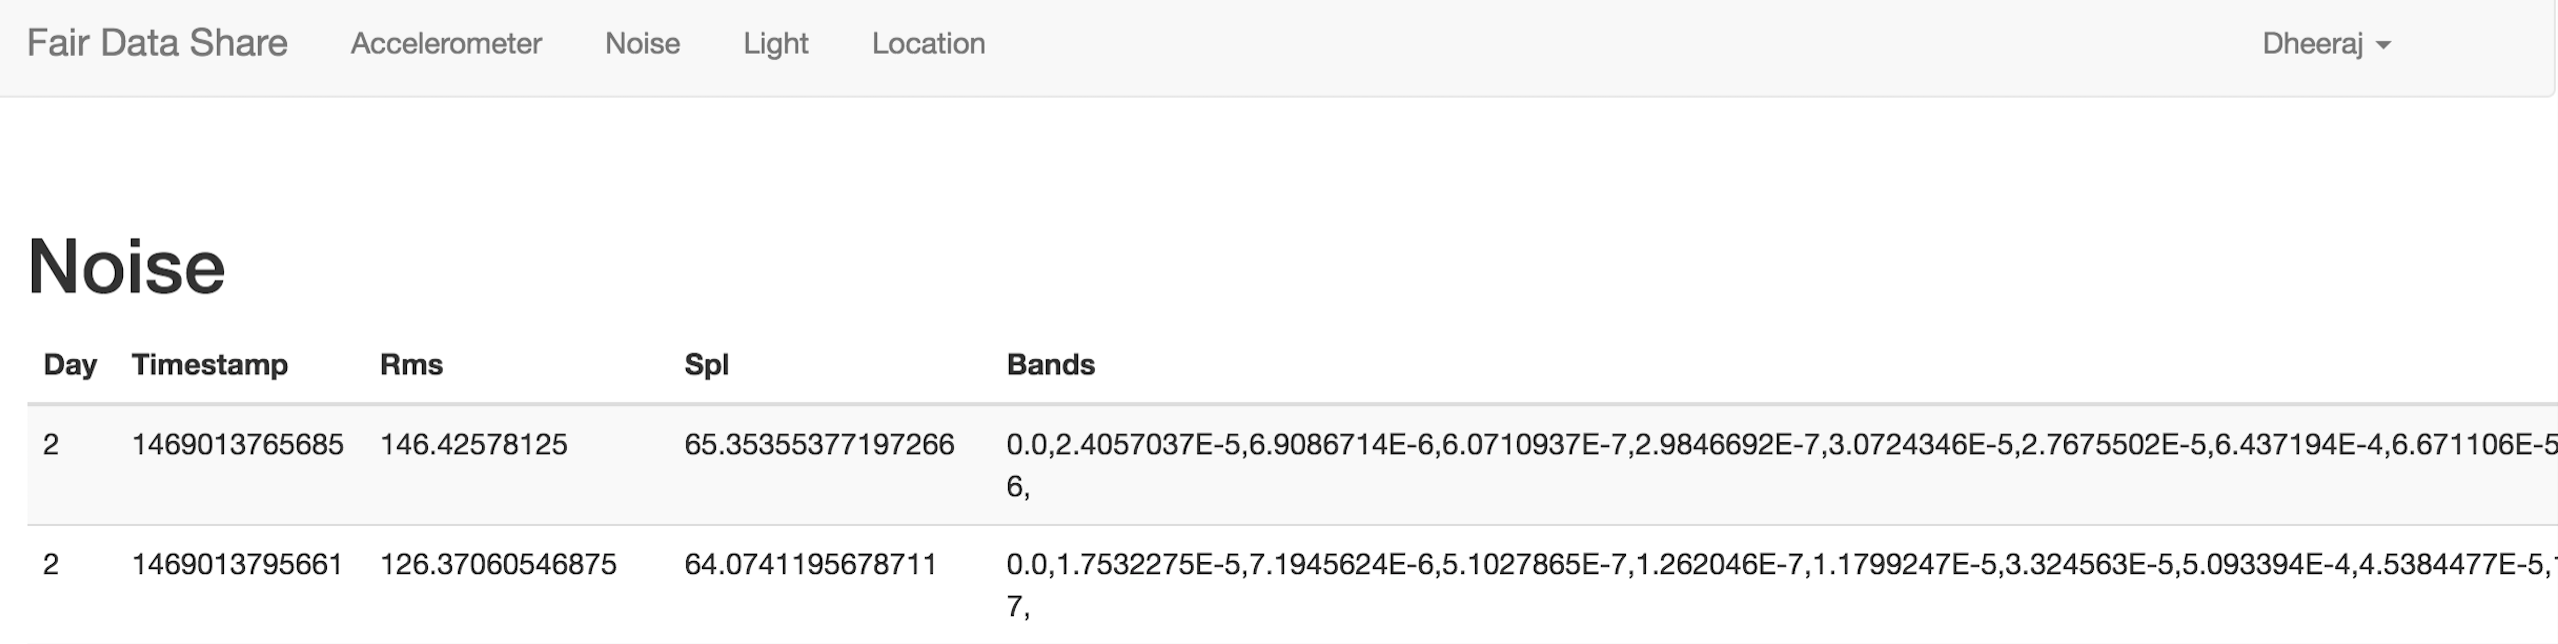
\includegraphics[width=0.4\linewidth]{./images/fds_user_noise_full}}%
  \caption{User Data}
  \label{fig:fds3}
\end{figure}




\subsection{Stakeholder's Portal}

For a stakeholder to view data, they need to register in the portal shown in figure \ref{fig:fds_home} by clicking register. Once that is done,
the page in figure \ref{fig:fdsdcregister} is shown asking for the following details :

\begin{enumerate}
    \item Company Name
    \item Email
    \item Stakeholder Category
    \item Company Website
\end{enumerate}

The stakeholder category is the type the stakeholder comes under such as :

\begin{enumerate}
    \item Corporation
    \item Educational Institution
    \item Government
    \item Non-Governmental Organization
\end{enumerate}


Once these details have been filled in, the stakeholder can click on the register button. Once registered, the stakeholder can login like shown in figure \ref{fig:fdsdclogin}.When access is granted the stakeholder is redirected to the page shown in figure \ref{fig:fds5}. The stakeholder can choose from each of the available drop down lists :
\begin{enumerate}
    \item A sensor
    \item A context
    \item An anonymous user
    \item A bidding day number
\end{enumerate}

Once this is entered, the stakeholder can seethe  data for that user with the privacy level decided by the anonymous user. If the stakeholder does not see any data, it means the user did not share data for this particular request. Stakeholders can view the sensor data in a similar fashion to users shown in figures \ref{fig:fds2} and \ref{fig:fds3}. Data is available to the stakeholders 24 hours after the start of the core phase.


\begin{figure}[htp]
  \subtop[ Registration Page\label{fig:fdsdcregister}]{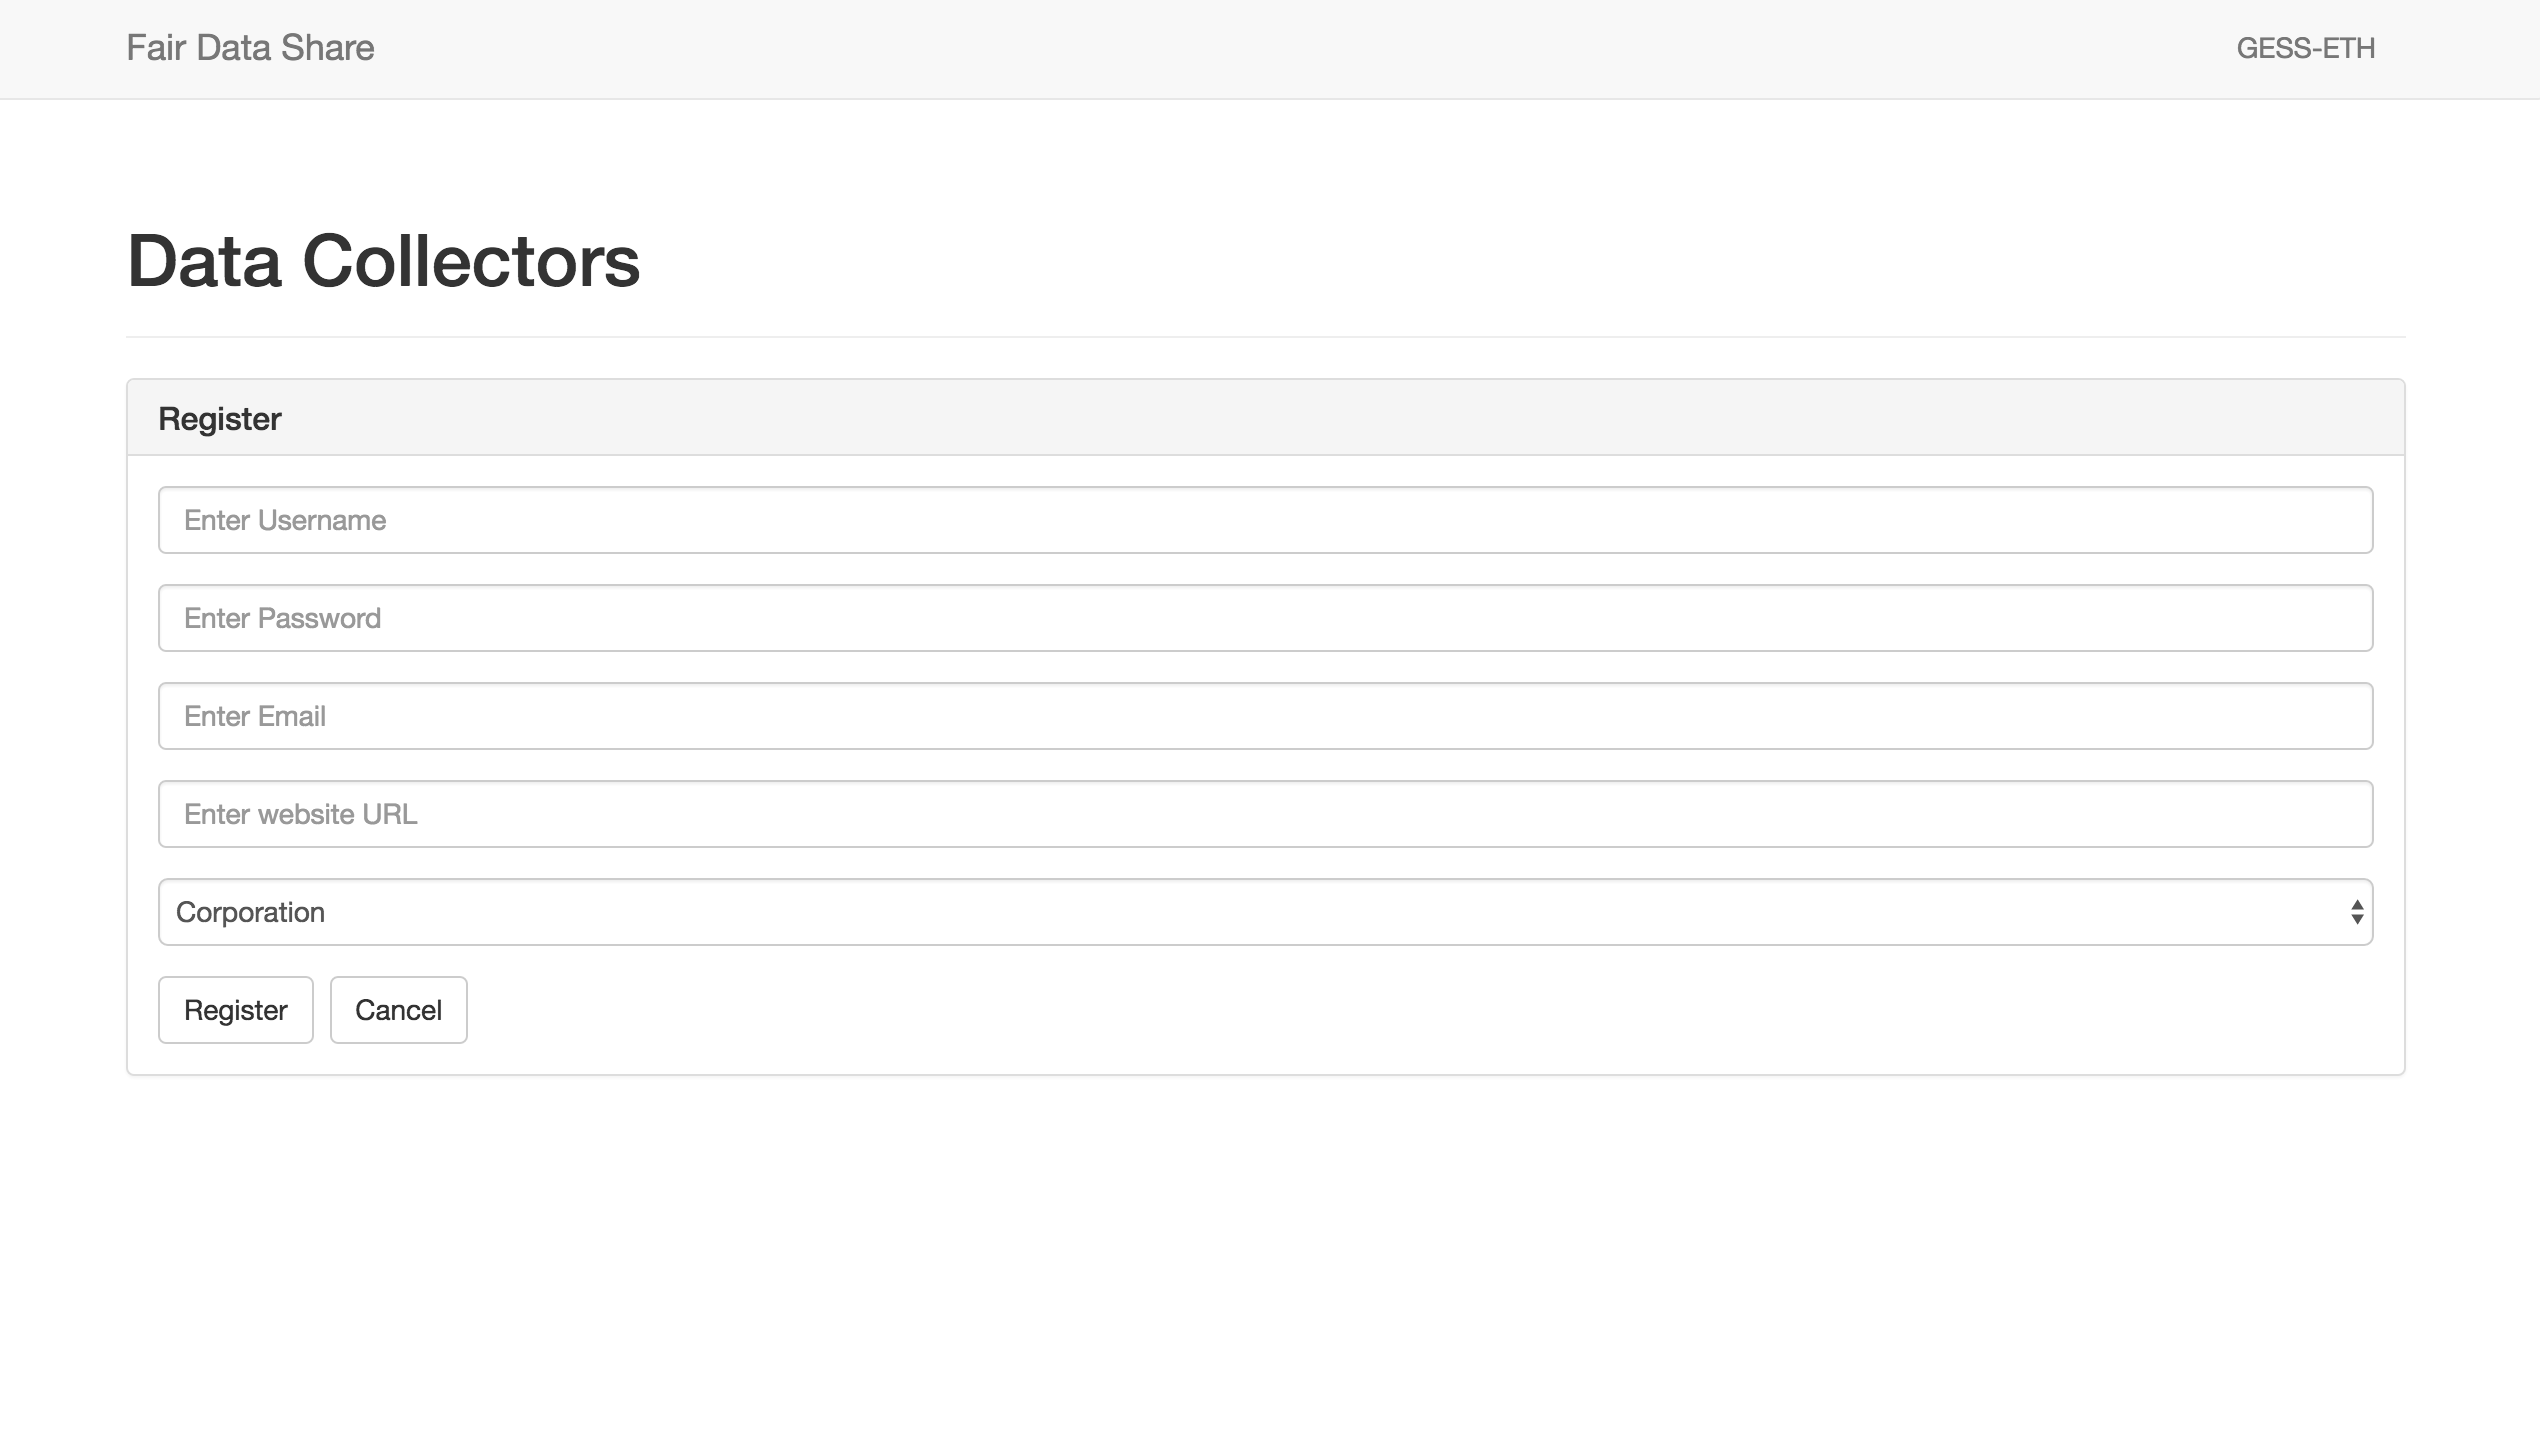
\includegraphics[width=0.4\linewidth]{./images/fds_dc_register}}\hspace{1em}
  \subtop[ Login Page\label{fig:fdsdclogin}]{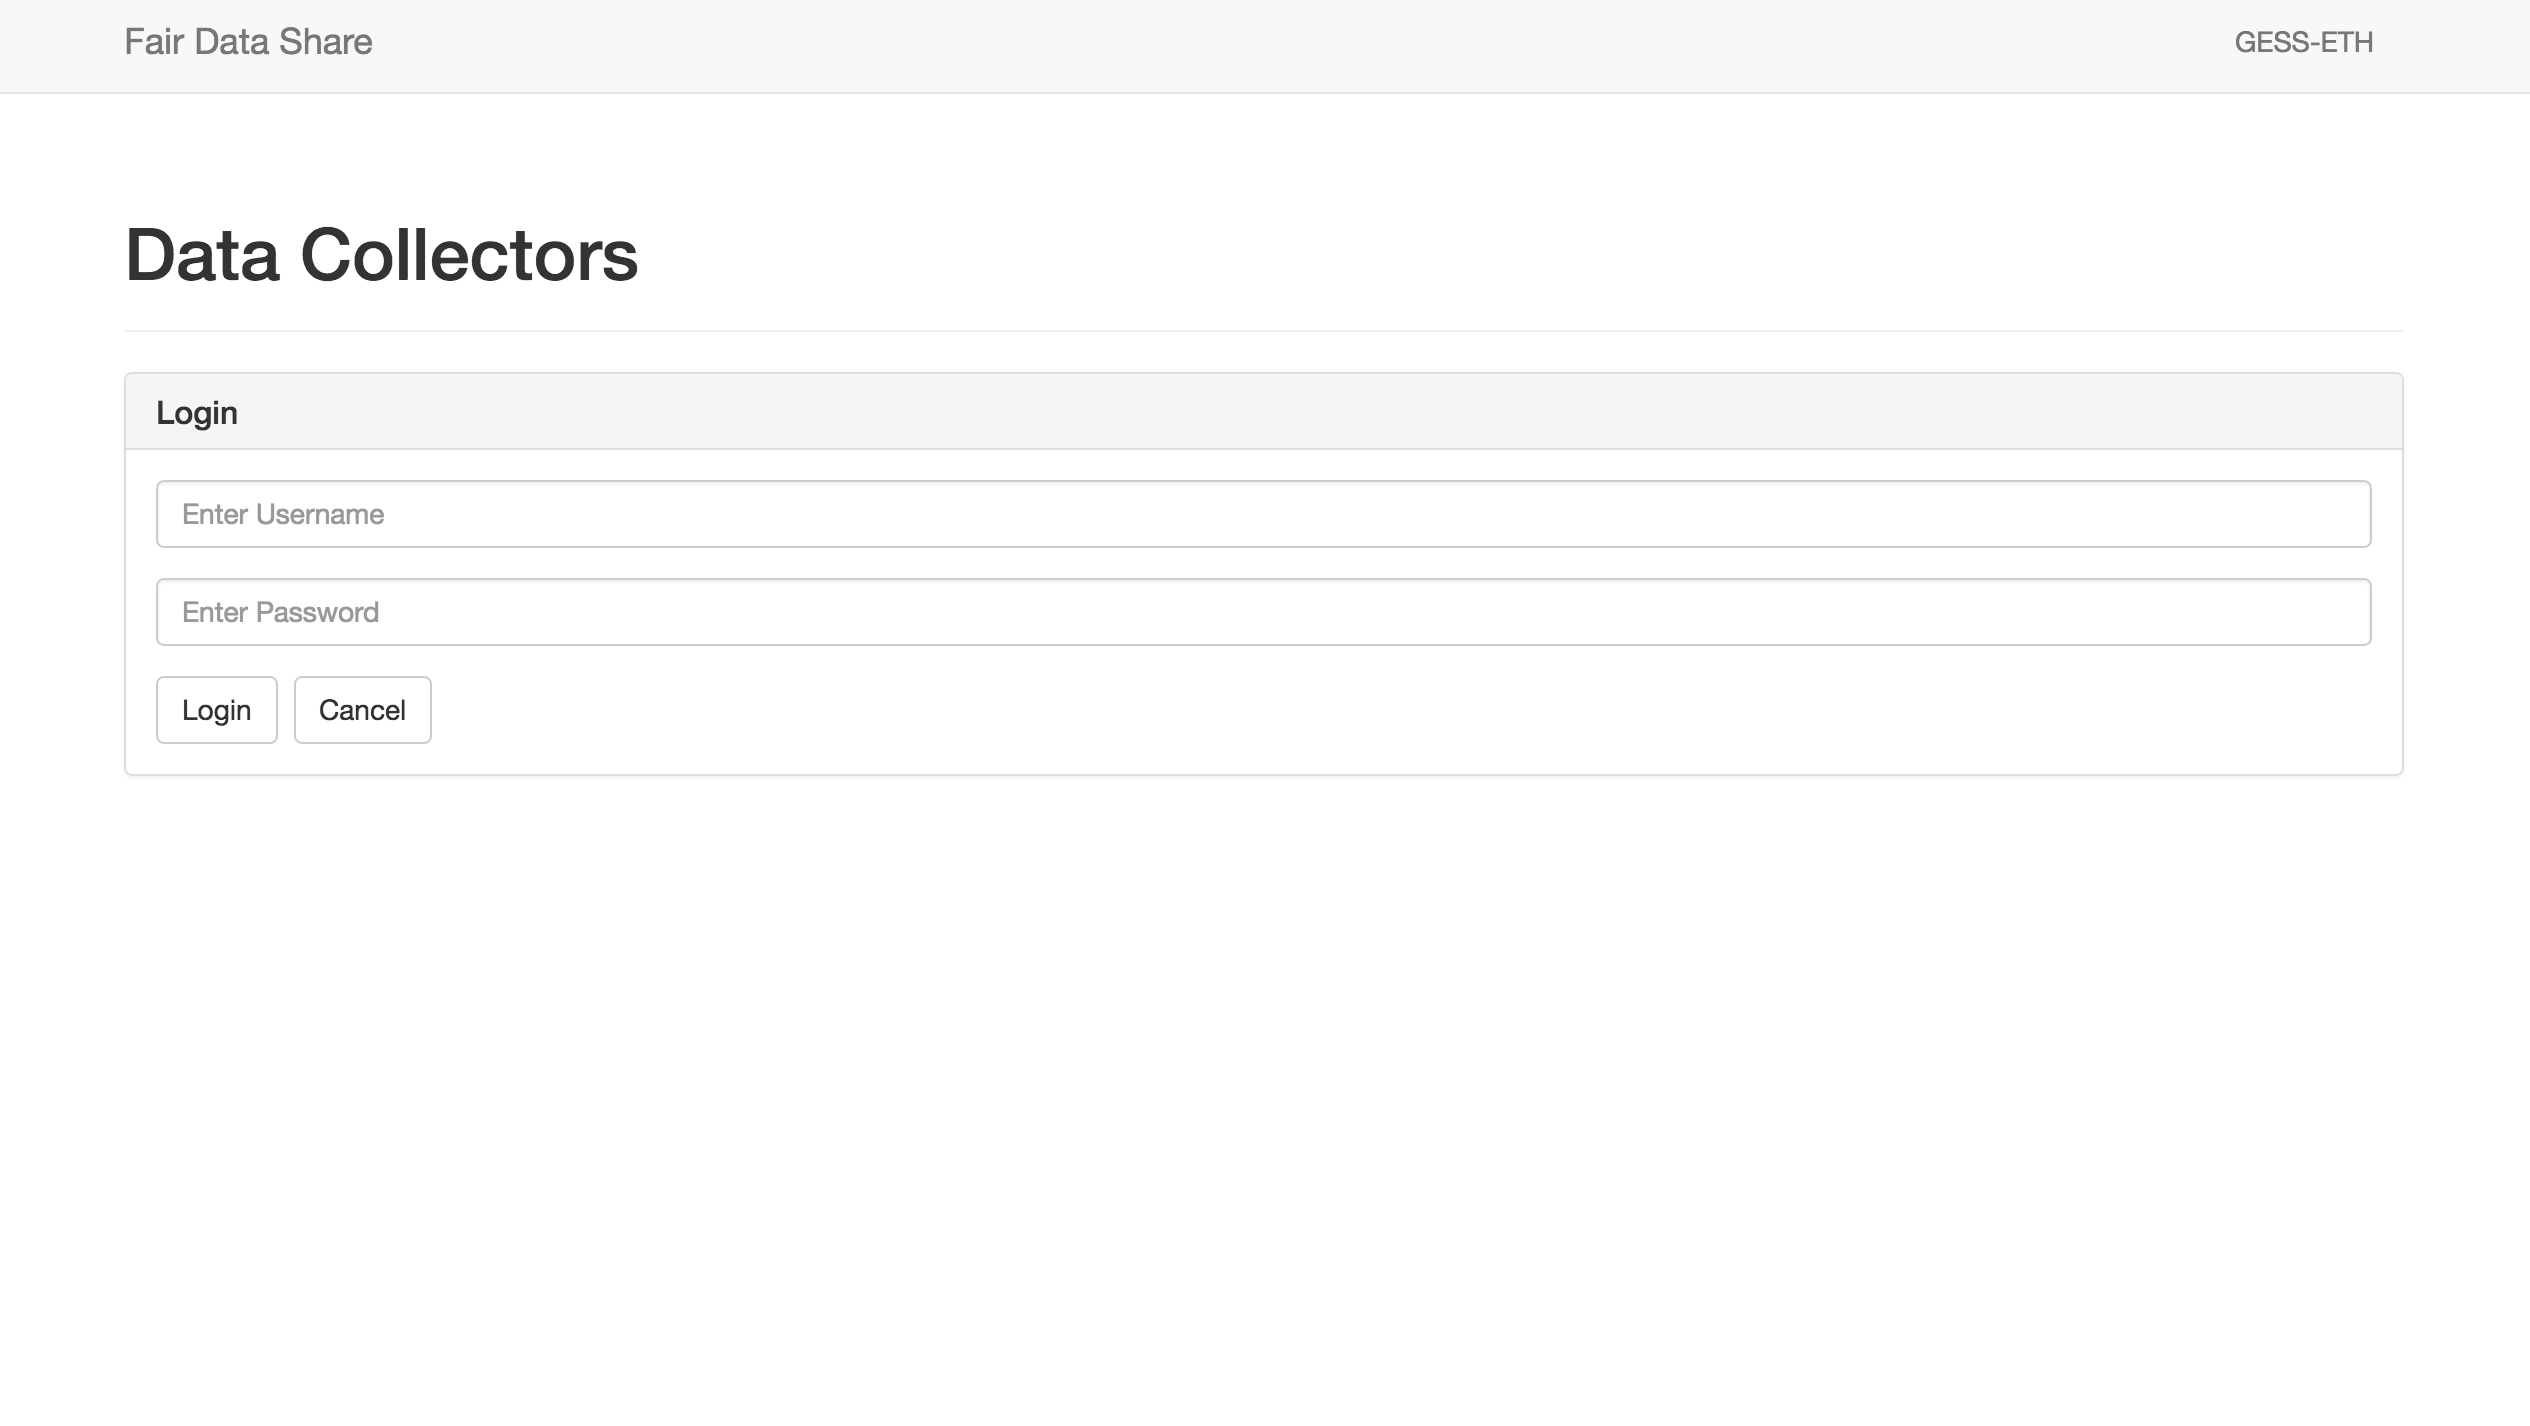
\includegraphics[width=0.4\linewidth]{./images/fds_dc_login}}%
  \caption{Entering the Portal for Data Collectors}
  \label{fig:fds4}
\end{figure}

\begin{figure}[ht!]
\centering
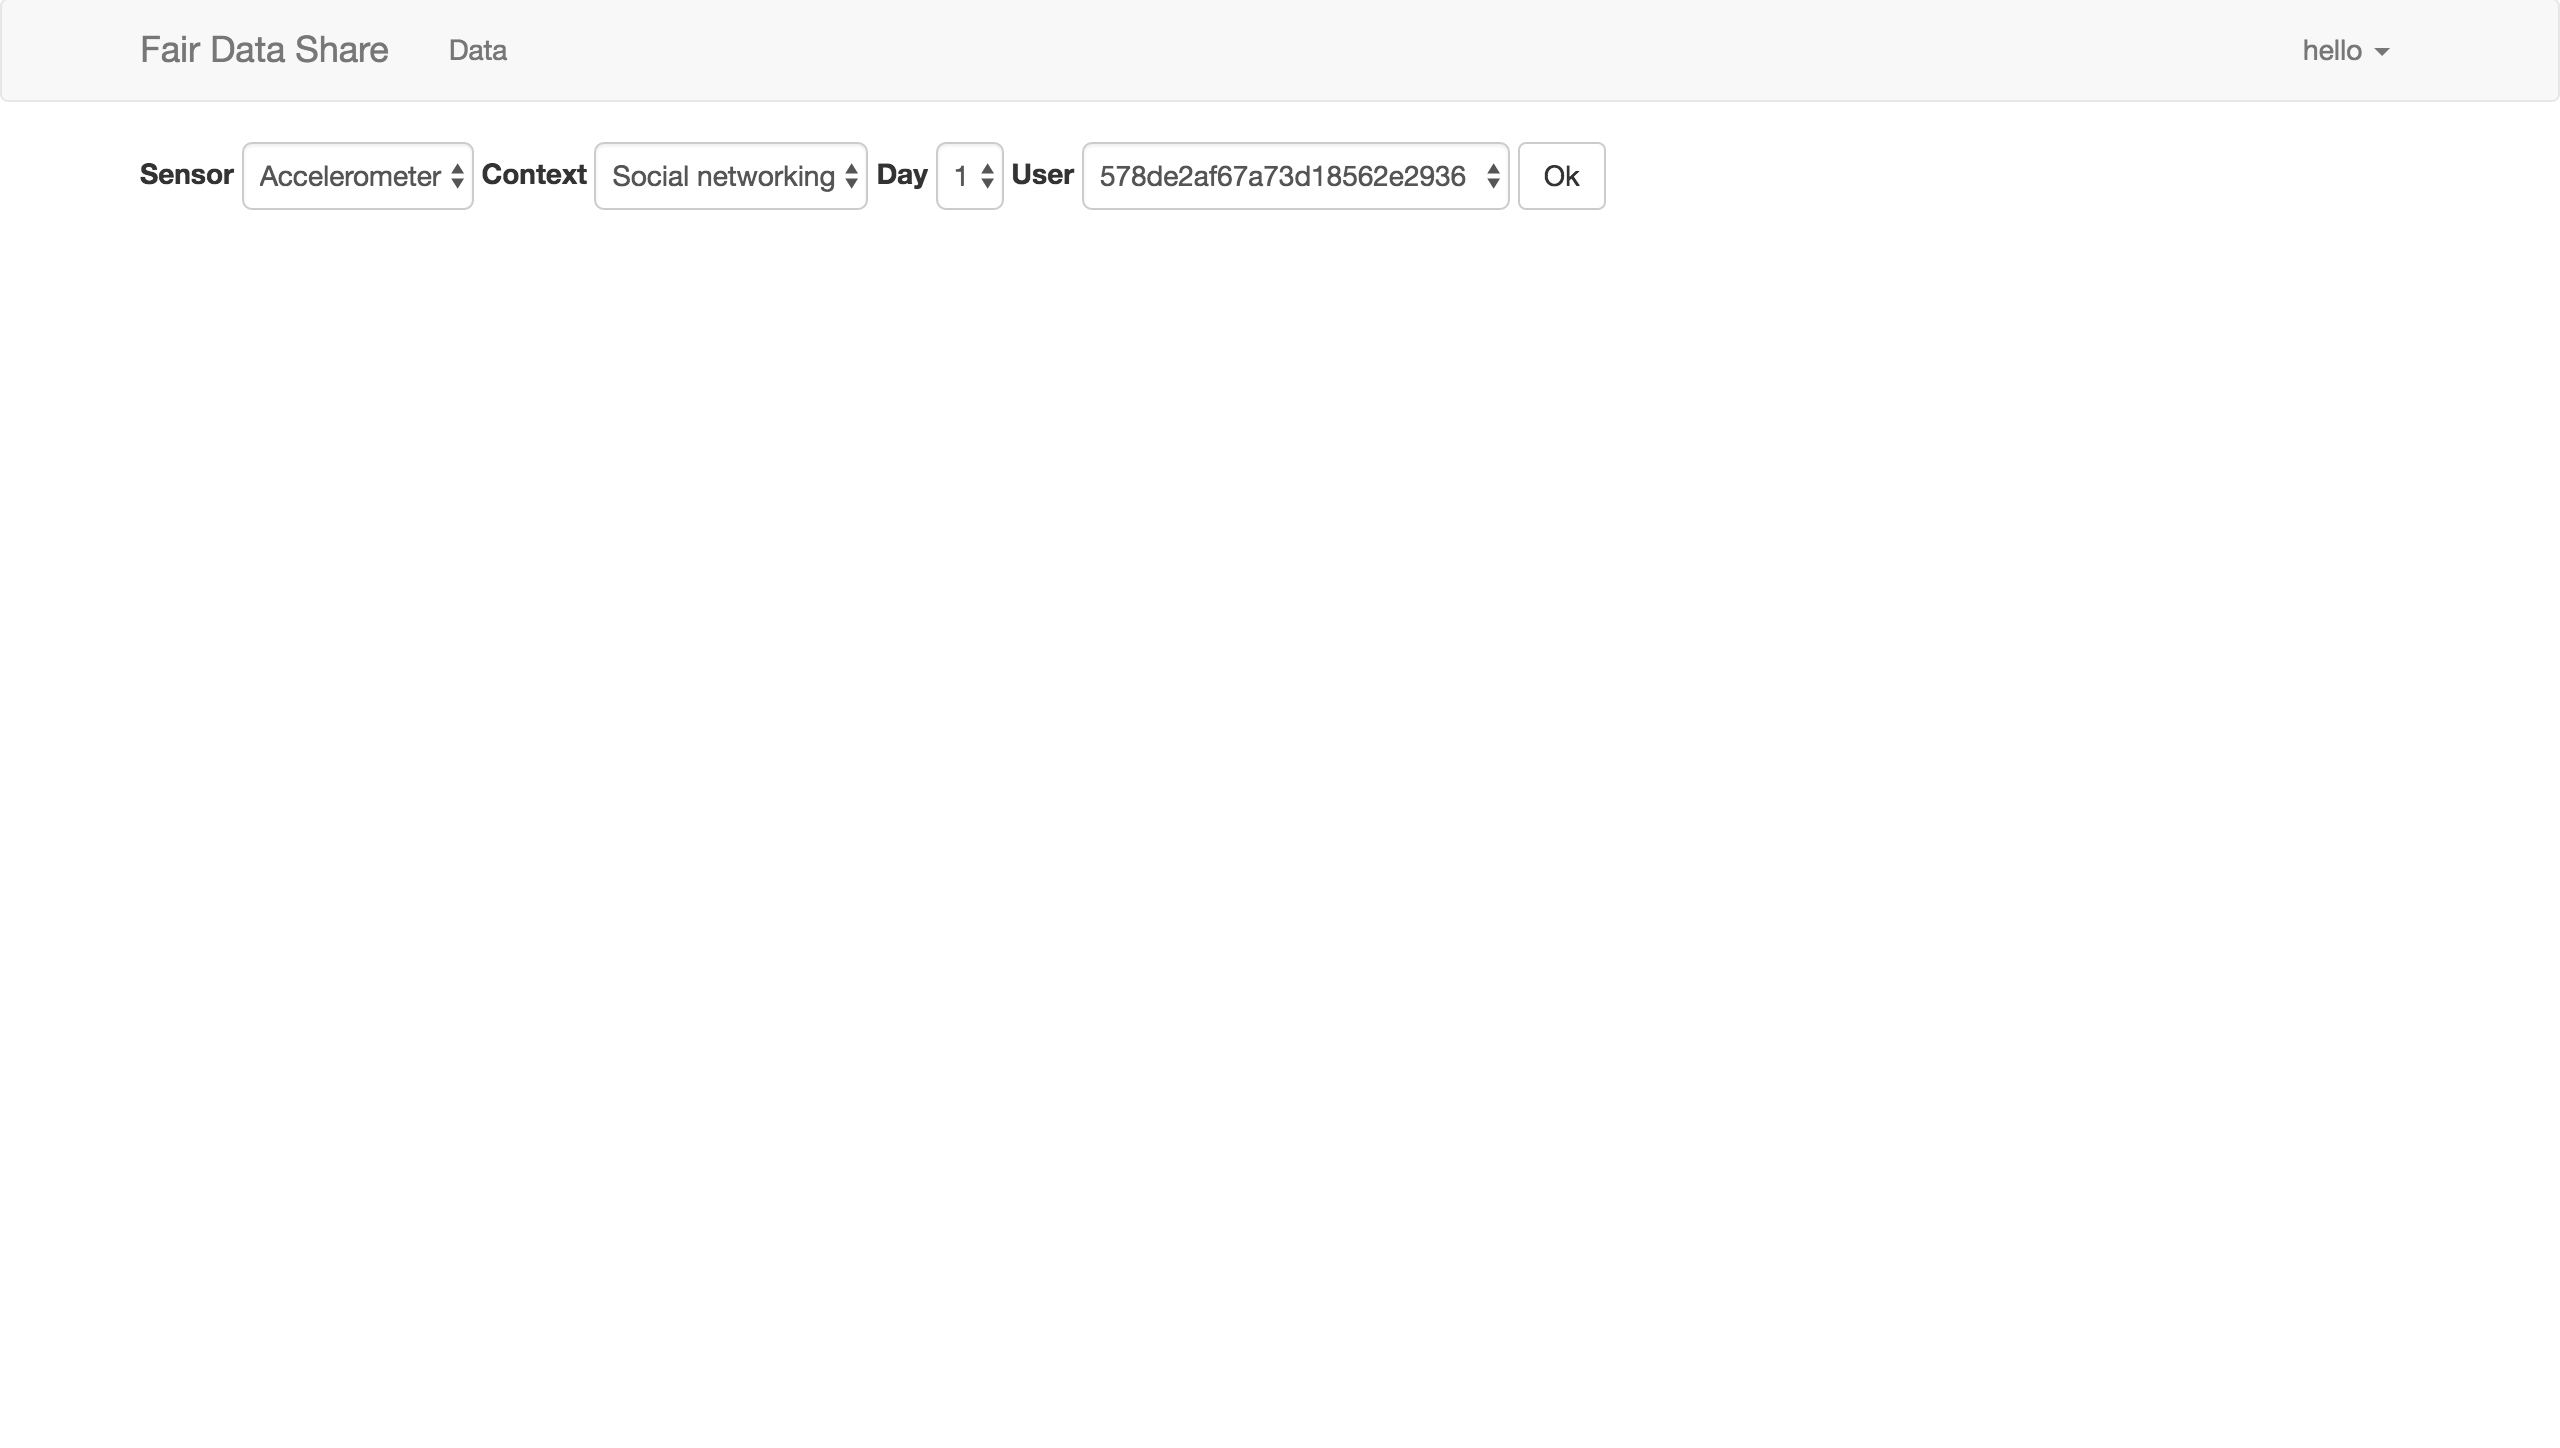
\includegraphics[width=\textwidth,keepaspectratio]{./images/fds_dc_welcome}
\caption{Data Collectors Welcome Page \label{fig:fds5}}
\end{figure}






